% T12 C/D, chapitre 9 : Limites, continuité et dérivation. Source : le livre « Terminales scientifiques » (Fonction/Lesona, Fonction/Fiche, Fonction/Exo).
% Les exercices tirés d’autres ouvrages ne sont pas repris (décision du 2 novembre 2026).

\TCDLessonStyleOn
\newcommand{\Df}{\mathcal{D}_f}

\chapter{G\'en\'eralit\'es sur les fonctions}
\section{Limites et continuit\'e}
      \begin{prop}[Limites aux infinis]
      \index{Limites!infinis}
            Les limites aux infinis se calculent de mani\`ere similaire \`a celles des suites.
            
            La limite en $\pm\infty$ d'une fraction rationnelle est \'egale \`a la limite du quotient des termes de plus haut degr\'e.
            \begin{ex}
                  \[
                  \lim_{x\rightarrow+\infty} \frac{x^3-23x^2+37}{-2x^2-57} = \lim_{x\rightarrow+\infty} \frac{x^3}{-2x^2} 
                                                                           = \lim_{x\rightarrow+\infty} \frac{x}{-2}      
                                                                           = -\infty	.
                  \]
            \end{ex}
      \end{prop}
%
      \begin{defi}[Limites en $x_0$]
      \index{Limites!en x0@en $x_0$}
            Soient $f$ une fonction et $x_0$ un nombre r\'eel.
            \begin{itemize}
                  \item On dit que $f$ tend vers $+\infty$ quand $x$ tend vers $x_0$ si 
                        $f(x)$ devient positif et aussi grand que l'on veut
                        d\`es que $x$ est suffisamment proche de $x_0$.
                  \item On dit que $f$ tend vers $-\infty$ quand $x$ tend vers $x_0$ si 
                        $f(x)$ devient n\'egatif et aussi grand que l'on veut en valeur absolue
                        d\`es que $x$ est suffisamment proche de $x_0$.
                  \item On appelle \emph{limite de $f$ \`a gauche de $x_0$} 
                     \index{Limites!en x0@en $x_0$!a gauche@\`a gauche}
                        la limite de $f$ quand $x$ tend vers ${x_0}$ par valeur inf\'erieure.
                        On note 
                        \begin{center}
                              \defbox{$\displaystyle{ \lim_{\substack{x\rightarrow x_0\\x<x_0}} f(x) }$}
                              ou encore \defbox{$\displaystyle{ \lim_{x\rightarrow {x_0}^-} f(x) }$}.
                        \end{center}
                  \item On appelle \emph{limite de $f$ \`a droite de ${x_0}$} 
                     \index{Limites!en x0@en $x_0$!a droite@\`a droite}
                        la limite de $f$ quand $x$ tend vers ${x_0}$ par valeur sup\'erieure.
                        On note 
                        \begin{center}
                              \defbox{$\displaystyle{ \lim_{\substack{x\rightarrow {x_0}\\x>{x_0}}} f(x) }$}
                              ou encore \defbox{$\displaystyle{  \lim_{x\rightarrow {x_0}^+} f(x) }$}.
                        \end{center}
            \end{itemize}
%
      \begin{rmk}~\\[-1\baselineskip]
            \begin{itemize}
            \item Il est possible que $\lim_{x\rightarrow a^+} f(x)$ soit diff\'erente de $\lim_{x\rightarrow a^-} f(x)$.
            \item Si $\lim_{x\rightarrow a^+} f(x) = \ell = \lim_{x\rightarrow a^-} f(x)$ 
                  alors $\lim_{x\rightarrow a} f(x)$ existe et est \'egale \`a $\ell$.
            \end{itemize}
      \end{rmk}
      \end{defi}
%
      \begin{defi}[Asymptotes]
      \index{Courbe!Branches infinies!Asymptotes}
            Soit $f$ une fonction.
            
            Si $\lim_{x\rightarrow+\infty}f(x)=b$ (ou $\lim_{x\rightarrow-\infty}f(x)=b$), avec $b$ r\'eel,
            la droite d'\'equation $y=b$ est alors appel\'ee une \emph{asymptote horizontale}
            \`a la courbe repr\'esentative de $f$.
            \index{Courbe!Asymptotes!horizontales}
            
            Si $\lim_{x\rightarrow {a}^{+}}f(x)$ ou $\lim_{x\rightarrow {a}^{-}}f(x)$ est infinie ($+\infty$ ou $-\infty$),
            la droite d'\'equation $x=a$ est alors appel\'ee une \emph{asymptote verticale}
            \`a la courbe repr\'esentative de $f$.
            \index{Courbe!Asymptotes!verticales}
            \begin{ex}~\\
                  \begin{figure}[H]
                  \centering
                        \begin{tikzpicture}[line cap=round,line join=round,>=stealth]
                        \Milimetre{(-5.14,-1.19)}{(5.23,2.23)}
                        \draw[->,color=black,thick] (-5.14,0) -- (5.23,0);
                        \foreach \x in {-5,-4,-3,-2,-1,1,2,3,4,5}
                        \draw[shift={(\x,0)},color=black] (0pt,2pt) -- (0pt,-2pt) node[below] {\footnotesize $\x$};
                        \draw[->,color=black,thick] (0,-1.19) -- (0,2.23);
                        \foreach \y in {-1,1,2}
                        \draw[shift={(0,\y)},color=black] (2pt,0pt) -- (-2pt,0pt) node[left] {\footnotesize $\y$};
                        \draw[color=black] (0pt,0pt) node[above right] {\footnotesize $0$};
                        \clip(-5.14,-1.19) rectangle (5.23,2.23);
                        \draw [color=loko1,domain=-5.14:5.23, thick] plot(\x,{(--1-0*\x)/1});
                        \draw[color=loko2, smooth,samples=100,domain=-5.14:5.23, very thick] plot(\x,{1-(2*(\x)-1)/((\x)^4+1+2.718^(-(\x)))});
                        \draw[color=loko2] (5,1) node[below] {\footnotesize $\mathscr{C}$};
                        \draw[color=loko1] (-5,1) node[below] {\footnotesize $\mathscr{D}$};
                        \end{tikzpicture}
                        \caption{Dans cet exemple, $\lim_{x\rightarrow-\infty}f(x)=\lim_{x\rightarrow+\infty}f(x)=1$.
                                 La droite $(\mathscr{D})$ est une asymptote horizontale.
                                 On constate que la courbe $\mathscr{C}$ s'approche de $(\mathscr{D})$.
                                 Remarquez que la courbe \emph{peut} couper l'asymptote!
                                 }
                        \label{fig:asymptote horizontale}
                  \end{figure}
                  %%%%%%%%%%%%%%%%%%%%%%%%%%%%%%%%%%%
                  \begin{figure}[H]
                  \centering
                        \caption{%
                                 Dans cet exemple, $\lim_{x\rightarrow 1^-}f(x)=-\infty$ et
                                 $\lim_{x\rightarrow 1^+}f(x)=+\infty$.
                                 La droite $(\mathscr{D})$ est une asymptote verticale.
                                 On constate que la courbe $\mathscr{C}$ s'approche de $(\mathscr{D})$.
                             }
                        \begin{tikzpicture}[>=stealth]
                        \Milimetre{(-2.25,-2)}{(4,3)}
                        \draw[->,color=black,thick] (-2,0) -- (4,0);
                        \foreach \x in {-2,-1,1,2,3}
                        \draw[shift={(\x,0)},color=black] (0pt,2pt) -- (0pt,-2pt) node[below] {\footnotesize $\x$};
                        \draw[->,color=black,thick] (0,-3) -- (0,3);
                        \foreach \y in {-2,-1,1,2,3}
                        \draw[shift={(0,\y)},color=black] (2pt,0pt) -- (-2pt,0pt) node[left] {\footnotesize $\y$};
                        \draw[color=black] (0pt,0pt) node[above right] {\footnotesize $0$};
                        \draw [color=loko1, thick] (1,-3.36) -- (1,4.14);
                        \draw[color=loko2, smooth,samples=500,domain=-3.164:0.99, very thick] plot(\x,{(\x)^3/(9*((\x)-1))});
                        \draw[color=loko2, smooth,samples=500,domain=1.01:4.14, very thick] plot(\x,{(\x)^3/(9*((\x)-1))});
                        \draw[color=loko2] (1,3.5) node[right] {\footnotesize $\mathscr{C}$};
                        \draw[color=loko1] (1,-2.5) node[right] {\footnotesize $\mathscr{D}$};
                        \end{tikzpicture}
                        \label{fig:asymptote verticale}
                  \end{figure}
            \end{ex}
      \end{defi}

      \begin{prop}
      \index{Limites!operations sur@op\'erations sur}
      Les op\'erations sur les limites se font comme d'habitude :
            \begin{table}[H]
            \centering
            \begin{tabular}{|c|c|c|}
            \hline 
                  \headingstyleko
            $\lim f$ & $\lim g$ & $\lim (f+g)$ \\ 
            \hline 
            $\ell$ & $\ell'$ & $\ell+\ell'$ \\ 
            \hline 
            $\ell$ & $+\infty$ & $+\infty$ \\ 
            \hline 
            $\ell$ & $-\infty$ & $-\infty$ \\ 
            \hline 
            $+\infty$ & $+\infty$ & $+\infty$ \\ 
            \hline 
            $-\infty$ & $-\infty$ & $-\infty$ \\ 
            \hline 
            $+\infty$ & $-\infty$ & Forme ind\'etermin\'ee \\ 
            \hline 
            \end{tabular} 
            \index{Limites!operations sur@op\'erations sur!somme}
            \caption{Limite d'une somme.}
            \label{tab:limite somme}
            \end{table}
            %
%            \begin{minipage}{.45\textwidth}
            \begin{table}[H]
            \centering
            \begin{tabular}{|c|c|c|}
            \hline 
                  \headingstyleko
            $\lim f$ & $\lim g$ & $\lim (f\cdot g)$ \\ 
            \hline 
            $ \ell $ & $ \ell' $ & $ \ell \cdot \ell' $ \\
            \hline
            $ \ell (\neq 0) $ & $ \infty $ & $\infty$ (signe du produit) \\
            \hline 
            $ \infty $ & $\infty $ & $\infty $ (signe du produit) \\
            \hline 
            $0$ & $\infty$ & Forme ind\'etermin\'ee \\
            \hline                                     
            \end{tabular} 
                  \index{Limites!operations sur@op\'erations sur!produit}
            \caption{Limite d'un produit.}
            \label{tab:limite produit}
            \end{table}
%            \end{minipage}
            %
%            \begin{minipage}{.45\textwidth}
            \begin{table}[H]
            \centering
            \begin{tabular}{|c|c|c|}
            \hline 
                  \headingstyleko
            $\lim f$ & $\lim g$ & $\lim \left( \frac{f}{g} \right)$ \\ 
            \hline 
            $ \ell $ & $ \ell' (\neq 0) $ & $ \frac{\ell}{\ell'} $ \\
            \hline
            $ \ell $ & $\infty $ & $0$ \\
            \hline
            $ \ell (\neq 0) $ & $ 0 $ (avec $g$ de signe constant) & $\infty$ (r\`egle des signes) \\
            \hline 
            $ \infty $ & $ \ell' $ & $\infty $ (r\`egle des signes) \\
            \hline 
            $0$ & $0$ & Forme ind\'etermin\'ee \\
            \hline
            $\infty$ & $\infty$ & Forme ind\'etermin\'ee \\
            \hline                                     
            \end{tabular} 
                  \index{Limites!operations sur@op\'erations sur!quotient}
            \caption{Limite d'un quotient.}
            \label{tab:limite quotient}
            \end{table}            
%            \end{minipage}
      \end{prop}

      \begin{thm}[Limite d'une fonction compos\'ee]
\index{Limites!fonctions composees@fonctions compos\'ees}
\index{Fonctions composees@Fonctions compos\'ees!limite}
            Soient $f$ et $g$ deux fonctions et soit $h = g\circ f$, c'est-\`a-dire $h(x) = g\left( f(x) \right)$.
            Si \hypothesebox{$ \lim_{x\rightarrow x_0} f(x) = y_0 $} 
            et \hypothesebox{$ \lim_{x\rightarrow y_0} g(x) = z_0$} 
            alors \thmbox{$\displaystyle{\lim_{x\rightarrow x_0} h(x) = z_0} $}.
            
            \smallnota{Ici, $x_0$, $y_0$ et $z_0$ peuvent \^etre des nombres r\'eels ou infinis.}
            \begin{ex}
                  Soit $h(x) = \cos \left( \frac{1}{x^2 + 1} \right)$.
                  On veut calculer la limite de $h(x)$ quand $x$ tend vers $-\infty$.
                  
                  On pose $f(x) = \frac{1}{x^2 + 1}$ et $g(x) = \cos x$.
                  Il vient que $g\left(f(x)\right) = \cos \left( \frac{1}{x^2 + 1} \right)$.
                  
                  \[
                  \left.
                  \begin{matrix}
                        \displaystyle{\lim_{x\rightarrow-\infty} f(x) = 0} \\
                        \displaystyle{\lim_{x\rightarrow 0} g(x) = 1} \\
                  \end{matrix}
                  \right\rbrace 
                  \Rightarrow
                  \lim_{x\rightarrow-\infty} h(x) = 1
                  \]
                  \begin{figure}[H]
                  \centering
                        \begin{tikzpicture}[>=stealth]
                        \Milimetre{(-5.14,-1.19)}{(5.23,2.23)}
                        \draw[->,color=black,thick] (-5.14,0) -- (5.23,0);
                        \foreach \x in {-5,-4,-3,-2,-1,1,2,3,4,5}
                        \draw[shift={(\x,0)},color=black] (0pt,2pt) -- (0pt,-2pt) node[below] {\footnotesize $\x$};
                        \draw[->,color=black,thick] (0,-1.19) -- (0,2.23);
                        \foreach \y in {-1,1,2}
                        \draw[shift={(0,\y)},color=black] (2pt,0pt) -- (-2pt,0pt) node[left] {\footnotesize $\y$};
                        \draw[color=black] (0pt,0pt) node[above right] {\footnotesize $0$};
                        \clip(-5.14,-1.19) rectangle (5.23,2.23);
                        \draw[color=loko2, smooth,samples=200,domain=-5.14:5.23, thick] plot(\x,{cos((1/((\x)^2+1))*180/pi)});
                        \draw [color=loko1,domain=-5.14:5.23] plot(\x,{1});
                        \draw[color=loko2] (5,1) node[below] {\footnotesize $\mathscr{C}$};
                        \draw[color=loko1] (-5,1) node[below] {\footnotesize $\mathscr{D}$};
                        \end{tikzpicture}
                        \caption{Courbe de la fonction $h$ d\'efinie par $h(x) = \cos \left(\frac{1}{x^2+1}\right)$.
                                 }
                        \label{fig:fonction composee}
                  \end{figure}
            \end{ex}
      \end{thm}

      \begin{defi}[Continuit\'e]
      \index{Continuite@Continuit\'e}
            Soit $f$ une fonction d\'efinie sur un intervalle $I$ et soit $a \in I$.
            On dit que \emph{$f$ est continue en $a$} si 
                  \defbox{$\lim_{x\rightarrow a^-} f(x) = \lim_{x\rightarrow a^+} f(x) = f(a)$}.
            On dit que $f$ est continue sur $I$ si elle est continue en tout point de $I$.
            
            Soit $f$ une fonction d\'efinie \`a gauche et \`a droite de $a$, mais pas en $a$.
            Si
                  $\lim_{x\rightarrow a^-} f(x) = \lim_{x\rightarrow a^+} f(x) = \ell$ avec $\ell$ \emph{r\'eel}, 
            alors on peut \emph{prolonger $f$ par continuit\'e} en $a$ en posant $f(a) = \lim_{x\rightarrow a} f(x)$.
\index{Prolongement par continuite@Prolongement par continuit\'e}
                  \begin{figure}[H]
                  \centering
                        \begin{tikzpicture}[>=stealth]
                        \clip (-5,-0.5) rectangle (5,1.5);
                        \Milimetre{(-5.14,-1.19)}{(5.23,2.23)}
                        \draw[->,color=black,thick] (-5.14,0) -- (5.23,0);
                        \foreach \x in {-5,-4,-3,-2,-1,1,2,3,4,5}
                        \draw[shift={(\x,0)},color=black] (0pt,2pt) -- (0pt,-2pt) node[below] {\footnotesize $\x$};
                        \draw[->,color=black,thick] (0,-1.19) -- (0,1.5);
                        \foreach \y in {-1,1,2}
                        \draw[shift={(0,\y)},color=black] (2pt,0pt) -- (-2pt,0pt) node[left] {\footnotesize $\y$};
                        \draw[color=black] (0pt,0pt) node[above right] {\footnotesize $0$};
                        \clip(-5.14,-1.19) rectangle (5.23,2.23);
                        \draw[color=loko2, smooth,samples=200,domain=-5.14:5.23,very thick] 
                                                                   plot(\x,{sin(((\x))*180/pi)/(\x)});
                        \draw[color=loko2] (5,-0.5) node[below] {\footnotesize $\mathscr{C}$};
                        \filldraw [fill=white,draw=loko1] (0,1) circle (2.5pt);
                        \end{tikzpicture}
                        \caption{Courbe de la fonction $f$ d\'efinie par $f(x) = \frac{\sin (x)}{x}$.
                                 Cette fonction n'est pas d\'efinie en $0$,
                                 mais comme $\lim_{x\rightarrow 0} f(x) = 1$,
                                 on peut prolonger $f$ par continuit\'e en posant $f(0) = 1$.
                                 }
                        \label{fig:prolongement par continuite}
                  \end{figure}
      \end{defi}
      
      \begin{prop}\vspace{-1\baselineskip}
      \begin{itemize}
            \item Les fonctions polyn\^omiales ainsi que les fonction $\sin$ et $\cos$ sont continues.
            \item La fonction racine carr\'ee est continue sur $[0,+\infty[$ ; plus g\'en\'eralement, les fonctions usuelles sont continues sur leur ensemble de d\'efinition.
            \item Le produit et la somme de deux fonctions continues sont continus.
            \item Le quotient de deux fonctions continues est continu sur tout intervalle dans lequel le d\'enominateur ne s'annule pas.
            \item La compos\'ee de deux fonctions continues est continue.
      \end{itemize}
      
      \end{prop}

      \begin{thm}[\textbf{T}h\'eor\`eme des \textbf{V}aleurs \textbf{I}nterm\'ediaires]
\index{Theoreme@Th\'eor\`eme!Valeurs Intermediaires@Valeurs Interm\'ediaires}
\index{TVI}
            Soit $f$ une fonction continue sur un intervalle $[a,b]$.
            On note respectivement par $m$ et $M$ le minimum et le maximum de $f$ sur $[a,b]$.
            Alors, pour tout $y_0\in[m,M]$, il existe $x_0\in[a,b]$ tel que \thmbox{$f(x_0)=y_0$}.      

            En particulier, pour tout r\'eel $k$ compris entre $f(a)$ et $f(b)$, l'\'equation $f(x) = k$ admet au moins une solution dans $[a,b]$ ;
            si $f(a)$ et $f(b)$ sont de signes contraires, l'\'equation $f(x) = 0$ admet au moins une solution dans $[a,b]$.
      \end{thm}
      \begin{prop}[Comparaison et encadrement]
      \index{Limites!comparaison}
            Soient $f$, $g$, $h$ des fonctions d\'efinies au voisinage de $x_0$ ($x_0$ r\'eel ou infini).
            \begin{itemize}
                  \item Si $f(x) \leq g(x)$ au voisinage de $x_0$ et $\lim_{x_0} f = +\infty$, alors $\lim_{x_0} g = +\infty$
                        (de m\^eme, si $g \leq f$ et $\lim_{x_0} f = -\infty$, alors $\lim_{x_0} g = -\infty$).
                  \item (Th\'eor\`eme des gendarmes) Si $f(x) \leq g(x) \leq h(x)$ au voisinage de $x_0$ et
                        $\lim_{x_0} f = \lim_{x_0} h = \ell$ (r\'eel), alors $\lim_{x_0} g = \ell$.
            \end{itemize}
            Par exemple, $-\frac{1}{x} \leq \frac{\sin x}{x} \leq \frac{1}{x}$ pour $x > 0$, donc $\lim_{x\rightarrow+\infty} \frac{\sin x}{x} = 0$.
            On admet aussi $\lim_{x\rightarrow 0} \frac{\sin x}{x} = 1$.
      \end{prop}

      \begin{defi}[Bijective]
\index{Bijectivite@Bijectivit\'e}
            Soit $f : E \rightarrow F$ une fonction.
            On dit que $f$ est \emph{bijective} si : 
                  \begin{description}
                        \item[Injectivit\'e :] 
\index{Injectivite@Injectivit\'e}
                                               si $a_1$ et $a_2$ sont des \'el\'ements de $E$ tels que 
                                               $f(a_1) = f(a_2)$, alors $a_1=a_2$.
                        \item[Surjectivit\'e :]
\index{Surjectivite@Surjectivit\'e}
                                               pour tout $b\in F$, il existe $a\in E$ tel que $f(a)=b$.
                  \end{description}
      \end{defi}
      
      \begin{prop}
            Soit $f$ une fonction \hypothesebox{continue et strictement monotone} sur un intervalle $I$. \linebreak
            Alors \thmbox{$f$ r\'ealise une bijection} de $I$ vers $f(I)$.
            
            La fonction $f$ admet alors une fonction r\'eciproque $f^{-1} : f(I) \rightarrow I$.
\index{Fonction reciproque@Fonction r\'eciproque}
            Cette r\'eciproque $f^{-1}$ est aussi une bijection continue et strictement monotone.
            De plus, $f$ et $f^{-1}$ varient dans le m\^eme sens.
            Si $f$ est d\'erivable en $x_0 \in I$ avec $f'(x_0) \neq 0$, alors $f^{-1}$ est d\'erivable en $y_0 = f(x_0)$ et
            $\left(f^{-1}\right)'(y_0) = \frac{1}{f'(x_0)}$ ; si $f'(x_0) = 0$, la courbe de $f^{-1}$ a une tangente verticale au point d'abscisse $y_0$.
      \end{prop}

      \begin{cor}
\index{Bijectivite@Bijectivit\'e!continue et strictement monotone}
            Soit $f$ une fonction continue et strictement monotone sur un intervalle $[a,b]$.
            On note respectivement par $m$ et $M$ le minimum et le maximum de $f$ sur $[a,b]$.
            Alors, pour tout $y_0\in[m,M]$, il existe \emph{un unique} $x_0\in[a,b]$ tel que \thmbox{$f(x_0)=y_0$}.
      \end{cor}

\section{D\'erivation}
\index{Derivee@D\'eriv\'ee}
      \begin{defi}[D\'erivabilit\'e]
\index{Derivee@D\'eriv\'ee!en un point}
\index{Derivee@D\'eriv\'ee!sur un intervalle}
            Soient $f$ une fonction et $x_0 \in \mathbb{R}$.
            
            On dit que la fonction $f$ est d\'erivable au point $x_0$ si 
                  \defbox{   $ \lim_{x\rightarrow x_0} \frac{f(x) - f(x_0)}{x-x_0} $   }
            existe et est finie.
            Cette limite est appel\'ee \emph{nombre d\'eriv\'e} de $f$ en $x_0$ et est not\'ee \emph{$f'(x_0)$}.
            
            La fonction $f$ est dite d\'erivable sur un intervalle $]a,b[$ si elle est d\'erivable en tout point de $]a,b[$.
            L'application $f' : ]a,b[ \rightarrow \mathbb{R} , \ x \mapsto f'(x)$ est appel\'ee 
            \emph{fonction d\'eriv\'ee de $f$}.
            
            \smallnota{Toute fonction d\'erivable est aussi continue. Mais la r\'eciproque est fausse.}
      \end{defi}
      
      \begin{defi}[D\'erivabilit\'e \`a gauche et \`a droite]
\index{Derivee@D\'eriv\'ee!en un point!a gauche@\`a gauche}
\index{Derivee@D\'eriv\'ee!en un point!a droite@\`a droite}
            Soient $f$ une fonction et $x_0 \in \mathbb{R}$.
            On dit que la fonction $f$ est d\'erivable \`a gauche (resp. \`a droite) en $x_0$ si la fonction 
                  \defbox{$x \mapsto \frac{f(x)-f(x_0)}{x-x_0} $}
            admet une limite finie \`a gauche (resp. \`a droite).
            Cette limite est alors appel\'ee \emph{nombre d\'eriv\'e de $f$ \`a gauche (resp. \`a droite) en $x_0$}
            et not\'ee $f'_g (x_0)$ (resp. $f'_d (x_0)$ ).
            
            Si $f$ est une fonction de la variable $x$, sa d\'eriv\'ee par rapport \`a $x$ est aussi not\'ee 
                  \defbox{$\frac{\mathrm{d}f}{\mathrm{d}x}$}.
            
            \smallnota{$f$ est d\'erivable en $x_0$ si et seulement si $f$ est d\'erivable \`a gauche et \`a droite en $x_0$ avec $f'_g(x_0) = f'_d(x_0)$.
            Si $f'_g(x_0) \neq f'_d(x_0)$, le point de la courbe d'abscisse $x_0$ est un \emph{point anguleux} ;
            si le taux de variation tend vers l'infini, la courbe a une demi-tangente verticale.}
      \end{defi}
      
      \begin{defi}[D\'eriv\'ee successive]
\index{Derivee@D\'eriv\'ee!successive}
            Soit $f$ une fonction d\'erivable sur un intervalle $I$.
            Si $f'$ est aussi d\'erivable sur $I$, alors sa d\'eriv\'ee, 
            not\'ee $f''$ ou $\frac{\mathrm{d}^2f}{\mathrm{d}x^2}$ est appel\'ee
            \emph{d\'eriv\'ee seconde} de $f$ ; on dit que \emph{$f$ est deux fois d\'erivable} sur $I$.
            Plus g\'en\'eralement, si $f$ est $n$ fois d\'erivable sur $I$, 
            on note $f^{(n)}$ ou $\frac{\mathrm{d}^nf}{\mathrm{d}x^n}$
            sa d\'eriv\'ee $n^{\text{i\`eme}}$.
            Si $f$ admet une d\'eriv\'ee d'ordre $n$ pour tout $n\in \mathbb{N}^*$, alors $f$ est dite
            \emph{ind\'efiniment d\'erivable} sur $I$.
      \end{defi}
            
      \subsection{Interpr\'etation graphique de la d\'eriv\'ee}
\index{Derivee@D\'eriv\'ee!Interpretation graphique@Interpr\'etation graphique}
            Soient $f$ une fonction, 
            $\mathscr{C}$ la courbe repr\'esentative de $f$ 
            et $x_0\in \mathbb{R}$
            tels que $f'(x_0)$ existe.
            %
            Le nombre $f'(x_0)$ repr\'esente alors 
            le coefficient directeur de la droite $(\mathscr{T}_{x_0})$, 
            \emph{tangente} \`a $\mathscr{C}$ au point d'abscisse $x_0$.
            %
            L'\'equation de la droite $(\mathscr{T}_{x_0})$ peut s'\'ecrire
            \thmbox{$ y = f'(x_0) \cdot (x-x_0) + f(x_0) $}.

                  \begin{figure}[h!tb]
                  \centering
                        \begin{tikzpicture}[>=stealth,scale=2.5]
                        \clip(-1.5,-0.67) rectangle (1.71,1.9);
                        \coordinate (tl) at (-1.5,-0.67);
                        \coordinate (br) at (1.71,1.9);
                        \Milimetre{(br)}{(tl)}
                        \draw[->,color=black,thick] (-1.5,0) -- (1.71,0);
                        \foreach \x in {-1,1}
                        \draw[shift={(\x,0)},color=black] (0pt,2pt) -- (0pt,-2pt) node[below] {\footnotesize $\x$};
                        \draw[->,color=black,thick] (0,-0.67) -- (0,1.9);
                        \foreach \y in {,1,2}
                        \draw[shift={(0,\y)},color=black] (2pt,0pt) -- (-2pt,0pt) node[left] {\footnotesize $\y$};
                        \draw[color=black] (0pt,-10pt) node[right] {\footnotesize $0$};
                        \draw[color=loko2, smooth,samples=100,domain=-0.9999995023070956:1.7147589756629125, very thick] 
                                    plot(\x,{abs((\x))*sqrt((\x)+1)});
                        \draw [->,color=loko6, thick] (0,0) -- (0.6,0.6);
                        \draw [->,color=loko1, thick] (0,0) -- (-0.6,0.6);
                        \draw [->,color=loko1!50!loko4, thick] (-1,0) -- (-1,0.6);
                        \draw [<->,color=loko5, thick] (-1,0.39) -- (-0.35,0.39);
                        \end{tikzpicture}
                        \caption{Courbe avec ses demi-tangentes.
                              Ici, on a $f'_g(0) = -1$, $f'_d(0) = 1$ et $\lim_{x\rightarrow -1^+} f'(x) = +\infty$.
                              Noter que quand le taux de variation (ici la d\'eriv\'ee) tend vers l'infini, la tangente est verticale.
                              \`A l'inverse, quand la d\'eriv\'ee est nulle, la tangente est horizontale.
                                 }
                        \label{fig:demi-tangentes}
                  \end{figure}
            %
            \begin{prop}
                  Si $f$ est d\'erivable sur un intervalle $I$ et si $f'(x) > 0$ (resp. $f'(x)<0$) pour tout $x \in I$,
                  sauf peut-\^etre en un nombre fini de points o\`u $f'$ s'annule,
                  alors $f$ est strictement croissante (resp. strictement d\'ecroissante) sur $I$.
                  Si $f'(x) = 0$ pour tout $x \in I$, alors $f$ est constante sur $I$.
            \end{prop}
            %
                  \begin{thm}[\textbf{T}h\'eor\`eme des \textbf{A}ccroissements \textbf{F}inis]
\index{Theoreme@Th\'eor\`eme!Accroissement Finis}
\index{TAF}
                        Soient $a$ et $b$ deux nombres r\'eels tels que $a<b$.
                        Soit $f$ une fonction continue sur $[a,b]$ et d\'erivable sur $]a,b[$.
                        Alors il existe un r\'eel $c\in]a,b[$ tel que 
                              \thmbox{
                                    \[
                                          \frac{f(b)-f(a)}{b-a}=f'(c)
                                    \]
                              }.
                              \begin{figure}[H]
                              \centering
                                    \begin{tikzpicture}[>=stealth,x=1cm,y=.75cm]
                                    \clip(-5,-3.18) rectangle (2.87,2.08);
                                    \draw[smooth,samples=100,domain=-5.004308656164452:2.8695264419449] 
                                                                  plot(\x,{1/5*((\x)^3+3*(\x)^2-2*(\x)-5)});
                                    \draw [color=loko2,domain=-5:2.87]
                                                                  plot(\x,{(--1.92--3.01*\x)/5.55});
                                    \draw [dash pattern=on 1ex off 1ex,color=loko1,domain=-5:2.87] 
                                                                  plot(\x,{(-7.26--3.01*\x)/5.55});
                                    \fill [color=loko2] (-3.78,-1.7) circle (1.5pt);
                                    \draw[color=loko2] (-4,-1.5) node {$a$};
                                    \fill [color=loko2] (1.78,1.31) circle (1.5pt);
                                    \draw[color=loko2] (2,1) node {$b$};
                                    \fill [color=loko1] (0.61,-0.97) circle (1.5pt);
                                    \draw[color=loko1] (0.75,-1.25) node {$c$};
                                    \end{tikzpicture}                              
                              \caption{Il existe un point o\`u la pente de la tangente est \'egale \`a la pente de la corde.}
                              \label{fig:TAF}
                              \end{figure}
                  \end{thm}
            %
                  \begin{cor}[Th\'eor\`eme de ROLLE]
\index{Theoreme@Th\'eor\`eme!de ROLLE}
                        Soit $f$ une fonction continue sur $[a,b]$ et d\'erivable sur $]a,b[$.
                        Si $f(a) = f(b)$ alors il existe $c\in]a,b[$ tel que $f'(c) = 0$.
                  \end{cor}
            %
                  \begin{thm}[\textbf{I}n\'egalit\'e des \textbf{A}ccroissement \textbf{F}inis]
\index{Theoreme@Th\'eor\`eme!Accroissement Finis!In\'egalit\'e des}
\index{IAF}
                        Soit $f:[a,b]\rightarrow\mathbb{R}$ une fonction (avec $a$ et $b$ deux r\'eels tels que $a<b$).
                        Si 
                        \begin{itemize}
                              \item $f$ est \hypothesebox{continue sur $[a,b]$ et d\'erivable sur $]a,b[$}
                              \item il existe $M\in\mathbb{R}$ tel que \hypothesebox{$|f'(x)|\leq M$} pour tout $x\in]a,b[$
                        \end{itemize}
                        alors \thmbox{\[ \left| \frac{f(b) - f(a)}{b - a} \right| \leq M . \]}
                        Plus g\'en\'eralement, si $|f'(x)| \leq M$ sur un intervalle $I$, alors $|f(x) - f(y)| \leq M |x - y|$ pour tous $x$, $y$ de $I$ ;
                        et si $m \leq f'(x) \leq M$ sur $]a,b[$, alors $m(b-a) \leq f(b) - f(a) \leq M(b-a)$.
                  \end{thm}
            %
                  \paragraph{Application aux suites $u_{n+1} = f(u_n)$}
                  \index{Suites recurrentes@Suites r\'ecurrentes}
                        Soit $f$ une fonction d\'efinie sur un intervalle $I$ telle que $f(I) \subset I$, et $(u_n)$ d\'efinie par $u_0 \in I$ et
                        $u_{n+1} = f(u_n)$ ; alors $u_n \in I$ pour tout $n$ (r\'ecurrence).
                        \begin{itemize}
                              \item Si $(u_n)$ converge vers $\ell \in I$ et si $f$ est continue en $\ell$, alors $f(\ell) = \ell$ :
                                    la limite est une solution de l'\'equation $f(x) = x$.
                              \item Si $f(\ell) = \ell$ avec $\ell \in I$ et $|f'(x)| \leq k < 1$ sur $I$, l'in\'egalit\'e des accroissements finis donne
                                    $|u_{n+1} - \ell| \leq k\,|u_n - \ell|$, puis $|u_n - \ell| \leq k^n |u_0 - \ell|$ ; donc $(u_n)$ converge vers $\ell$.
                        \end{itemize}
            
            
      \subsection{D\'eriv\'ee usuelle}~\\[-1\baselineskip]
%      \begin{table}[H]
%      \centering
	      \begin{table}[H]
	            \begin{tabularx}{\linewidth}{|p{.2\linewidth}p{.2\linewidth}X|}
            \hline
                  \headingstyleko
            Fonctions      & D\'eriv\'ees & Domaines de d\'erivabilit\'es
            \\ \hline
            $c$    & $0$ & $\mathbb{R}$ 
            \\ \hline
            $\lambda x$    & $\lambda$ & $\mathbb{R}$ 
            \\ \hline
            $x^n$ ($n\in\mathbb{N}^*$)   & $n \cdot x^{n-1}$ & $\mathbb{R}$ 
            \\ \hline
            $\sqrt{x}$ & $\frac{1}{2\sqrt{x}}$ & $]0 ; +\infty [$
            \\ \hline
            $\frac{1}{x}$ & $-\frac{1}{x^2}$ & $]-\infty ; 0[ \cup ] 0 ; +\infty[$ 
            \\ \hline
            $\sin {x}$ & $\cos {x}$ & $\mathbb{R}$ 
            \\ \hline
            $\cos {x}$ & $-\sin {x}$ & $\mathbb{R}$ 
            \\ \hline
	            \end{tabularx}
         \caption{D\'eriv\'ee de fonctions usuelles.}
      \end{table}

      \begin{table}[H]
            \begin{tabular*}{.99\actualtextwidth}%
                        {| c e c e c |}
            \hline
                  \headingstyleko
            Fonctions      & D\'eriv\'ees & Domaines de d\'erivabilit\'es
            \\ \hline
            $\lambda u$    & $\lambda u'$ & en tout r\'eel o\`u $u$ est d\'erivable
            \\ \hline
            $u^n$ ($n\in\mathbb{N}^*$)   & $n \cdot u' \cdot u^{n-1}$ & en tout r\'eel o\`u $u$ est d\'erivable
            \\ \hline
            $\sqrt{u}$ & $\frac{u'}{2\sqrt{u}}$ & tout r\'eel o\`u $u$ est d\'erivable et strictement positif
            \\ \hline
            $\frac{1}{u}$ & $-\frac{u'}{u^2}$ & tout r\'eel o\`u $u$ est d\'erivable et diff\'erent de z\'ero
            \\ \hline
            $\sin {u}$ & $u' \cos {u}$ & en tout r\'eel o\`u $u$ est d\'erivable
            \\ \hline
            $\cos {u}$ & $- u' \sin {u}$ & en tout r\'eel o\`u $u$ est d\'erivable
            \\ \hline
            \end{tabular*}
         \caption{D\'eriv\'ees faisant intervenir des fonctions usuelles.}
      \end{table}

      \begin{table}[H]
            \begin{tabularx}{1\actualtextwidth}
                        {| Y  Y |}
            \hline
                  \headingstyleko Fonctions      & D\'eriv\'ees 
            \\ \hline
            $u + v$    & $u' + v'$
            \\ \hline
            $u\cdot v$    & $u' \cdot v + u \cdot v'$
            \\ \hline
            $\displaystyle{ \frac{u}{v} }$ & $\displaystyle{ \frac{u' \cdot v - u \cdot v'}{v^2} }$
            \\ \hline
            $\displaystyle{ f^{-1} }$    & $\displaystyle{ \frac{1}{f'\circ f^{-1}} }$ (l\`a o\`u $f'\circ f^{-1} \neq 0$)
\index{Fonction reciproque@Fonction r\'eciproque!derivee@d\'eriv\'ee}
            \\ \hline
            $f \circ g$    & $g' \cdot \left( f' \circ g \right)$
\index{Fonctions composees@Fonctions compos\'ees!derivee@d\'eriv\'ee}
            \\ \hline
            \end{tabularx}
         \caption{Op\'erations sur les d\'eriv\'ees.}
      \end{table}
%      \caption{Table de d\'eriv\'ees usuelle}
%      \index{Derivee@D\'eriv\'ee!table de}
%      \label{tab:derivee}
%      \end{table}

\section{Propri\'et\'es g\'eom\'etriques}
      \subsection{Sym\'etries}
\index{Courbe!Symetrie@Sym\'etrie}
            \begin{defi}[Fonction paire et impaire]
\index{Parite@Parit\'e}
                  Soit $f$ une fonction et $\Df$ son domaine de d\'efinition.
                  \begin{itemize}
                        \item Une fonction $f$ est dite paire si pour tout $x\in\Df$, on a $-x\in\Df$ et $f(-x) = f(x)$.
                        \item Une fonction $f$ est dite impaire si pour tout $x\in\Df$, on a $-x\in\Df$ et $f(-x) = -f(x)$.
                  \end{itemize}
            \end{defi}
            \subsubsection{Sym\'etrie par rapport \`a une droite verticale}
\index{Courbe!Symetrie@Sym\'etrie!par rapport a une droite@par rapport \`a une droite}
                  La courbe repr\'esentative d'une fonction paire admet une sym\'etrie par rapport \`a l'axe $Oy$.
                  Plus g\'en\'eralement, 
                  la courbe repr\'esentative d'une fonction $f$ admet une sym\'etrie
                  par rapport \`a la droite d'\'equation $x=a$ si
                  \[   \forall x\in\Df,\ (2a-x)\in\Df \text{ et } f(2a-x) = f(x)   \]
            \subsubsection{Sym\'etrie par rapport \`a un point}
\index{Courbe!Symetrie@Sym\'etrie!par rapport a un point@par rapport \`a un point}
                  La courbe repr\'esentative d'une fonction impaire admet une sym\'etrie par rapport \`a l'origine.
                  Plus g\'en\'eralement, 
                  la courbe repr\'esentative d'une fonction $f$ admet une sym\'etrie par rapport \`a un point $I = (a,b)$ si
                  \[   \forall x\in\Df,\ (2a-x)\in\Df \text{ et } f(2a-x) + f(x) = 2 b .  \]
      \subsection{P\'eriodicit\'e}
\index{Periodicite@P\'eriodicit\'e}
            Une fonction $f$ est dite p\'eriodique de p\'eriode $T$ si 
                  \[ \forall x \in \Df, x+T\in\Df \text{ et } f(x+T) = f(x)      \;. \]
            Les fonctions p\'eriodiques les plus fr\'equemment rencontr\'ees sont 
            les fonctions trigonom\'etriques $\sin$ et $\cos$ (de p\'eriode $2\pi$).
            
            Pour \'etudier une fonction p\'eriodique de p\'eriode $T$, 
            il suffit de l'\'etudier sur un intervalle de longueur $T$.
            Pour tracer la courbe, il suffit de le faire sur un tel intervalle,
            le reste de la courbe s'obtient par translation de cette partie.
      \subsection{Point d'inflexion}
\index{Courbe!Points d'inflexsion}
            Soient $I(a,b)$ un point et $f$ une fonction d\'efinie sur un voisinage de $a$.
            Notons par $(\mathscr{C})$ la courbe repr\'esentative de $f$.
            Le point $I$ de $(\mathscr{C})$ est un point d'inflexion si 
            la courbe $(\mathscr{C})$ traverse sa tangente au point $I$ (elle passe d'un c\^ot\'e \`a l'autre de cette tangente).
            
            Si $f$ est deux fois d\'erivable au voisinage du point $I$
            et si la d\'eriv\'ee seconde s'annule en $a$ en changeant de signe
            alors $I$ est un point d'inflexion.
                              \begin{figure}[h!t]
                              \centering
                                    \begin{tikzpicture}[>=stealth,x=7em,y=5em]
                                    \coordinate (I) at (0.67,0.47);
                                    \coordinate (txt) at (1.25,-0.25);
                                    \clip(-0.75,-0.65) rectangle (2.11,1.33);
                                    \draw[color=loko2, smooth,samples=100,domain=-0.7465507858958698:2.1134960912091096]
                                         plot(\x,{1/3*((\x)^3-2*(\x)^2+3*(\x))});
                                    \draw[color=loko1, smooth,samples=100,domain=-0.7465507858958698:2.1134960912091096]
                                         plot(\x,{(3*0.67^2-4*0.67+3)/3*((\x)-0.67)+1/3*(0.67^3-2*0.67^2+3*0.67)});
                                    \fill [color=loko6] (I) circle (2.5pt);
                                    \draw[color=loko6] (txt) node[below] {\textit{Point d'inflexion}};
                                    \draw[->] (txt) to[out=90,in=-60] (I);
                                    \end{tikzpicture}                              
                              \caption{Au point d'inflexion, la courbe traverse sa tangente.}
                              \label{fig:inflexion}
                              \end{figure}
      \subsection{Fonction r\'eciproque}
\index{Courbe!Fonction reciproque@Fonction r\'eciproque}
\index{Fonction reciproque@Fonction r\'eciproque!Courbe}
            Soit $f : E \rightarrow F$ une fonction bijective, notons par $\mathscr{C}$ sa courbe repr\'esentative.
            Elle admet alors une fonction r\'eciproque $f^{-1} : F \rightarrow E$ 
            dont on notera par $\mathscr{C}'$ la courbe repr\'esentative.
            Dans un rep\`ere orthonorm\'e, les courbes $\mathscr{C}$ et $\mathscr{C}'$ sont sym\'etriques par rapport \`a la premi\`ere bissectrice (droite d'\'equation $y = x$).
            %
            \begin{figure}[h!]
            \centering
		         \begin{tikzpicture}[line cap=round,line join=round,>=triangle 45,x=1.0cm,y=1.0cm]
		         \clip (-4,-4) rectangle (6,6);
	               \draw [color=black, xstep=.1,ystep=.1, opacity=.05, line width=.05] (-4,-4) grid (6,6);
	               \draw [color=black, xstep=.5,ystep=.5, opacity=.1, line width=.1] (-4,-4) grid (6,6);
	               \draw [color=black, xstep=1,ystep=1, opacity=.2, line width=.2] (-4,-4) grid (6,6);
		         \draw[->,color=black] (-4,0) -- (6,0);
		         \foreach \x in {-3,-2,-1,1,2,3,4,5}
		               \draw[shift={(\x,0)},color=black] (0pt,2pt) -- (0pt,-2pt) node[below] {\footnotesize $\x$};
		         \draw[->,color=black] (0,-4) -- (0,6);
		         \foreach \y in {-3,-2,-1,1,2,3,4,5}
		               \draw[shift={(0,\y)},color=black] (2pt,0pt) -- (-2pt,0pt) node[left] {\footnotesize $\y$};
		         \draw[color=black] (0pt,-10pt) node[right] {\footnotesize $0$};
		         \clip(-6,-6) rectangle (6,6);
		         \draw[color=loko2, smooth,samples=100,domain=-6:6] 
		               plot(\x,{((\x)-1)^3-1});
		         \draw (-6,-6) -- (6,6) node[very near end,sloped,below] {$y = x$} ;
		         \draw[color=loko1, smooth,samples=100,domain=-6:6] 
		               plot({((\x)-1)^3-1},\x);
		         \draw (5.5,0) node[above] {$x$};
		         \draw (0,5.5) node[right] {$y$};
		         \draw (-3.5,0) node[above] {$x'$};
		         \draw (0,-3.5) node[right] {$y'$};
		         \draw[color=loko2] (2,5.5) node[] {$y = f(x)$};
		         \draw[color=loko1 ] (5,2.5) node[] {$y = f^{-1} (x)$};
		         \end{tikzpicture}
	         \caption{Courbe d'une fonction trac\'ee dans le m\^eme rep\`ere que la courbe de sa fonction r\'eciproque.}
            \end{figure}
            %
\section{Branches infinies}
\index{Courbe!Branches infinies}
      Soient $f$ une fonction et $\mathscr{C}$ sa courbe repr\'esentative.
      La courbe $\mathscr{C}$ est alors un ensemble de points de la forme $(x,f(x))$.
      On parle de \emph{branche infinie} de la courbe quand au moins une des coordonn\'ees tend vers l'infini.
            
      On sait d\'ej\`a que si $\lim_{x\rightarrow x_0} f(x) = \infty$ (\`a gauche ou \`a droite) alors 
      la courbe $\mathscr{C}$ admet une asymptote verticale d'\'equation $x=x_0$.
\index{Asymptote!verticale}
      
      Pour ce qui est de la limite de $f(x)$ quand $x$ tend vers l'infini, il y a plusieurs possibilit\'es.
            \begin{figure}[h!]
            \centering
                  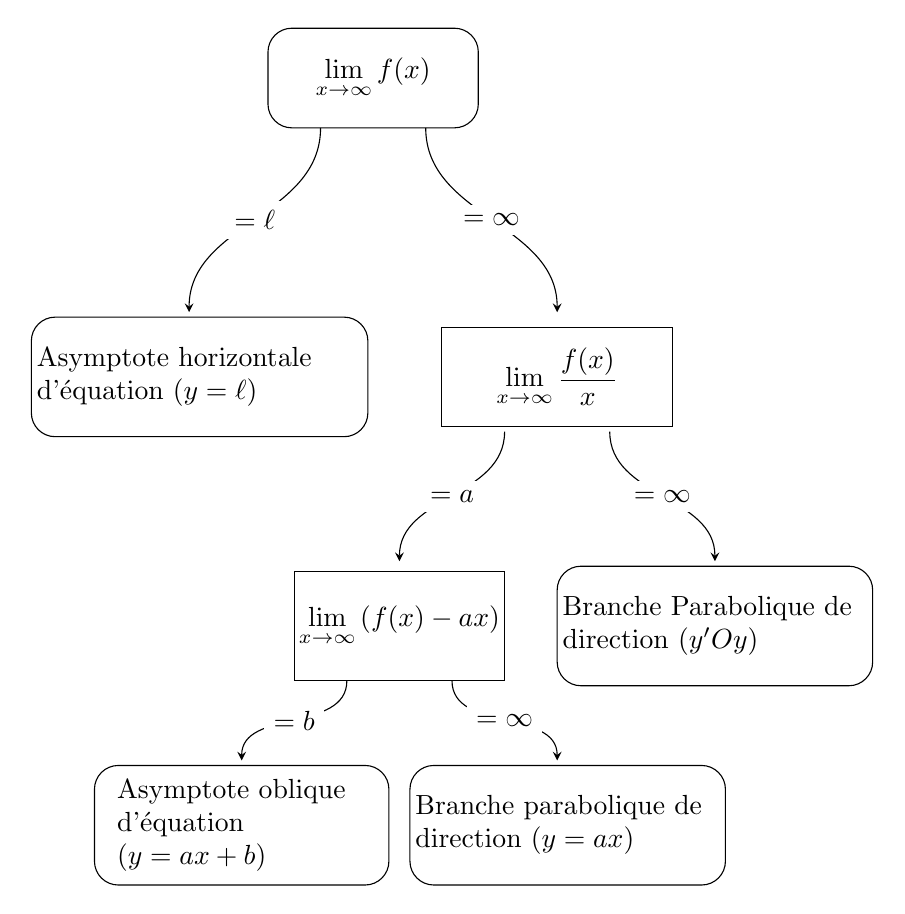
\begin{tikzpicture}[>=stealth,x=1.9em,y=3\baselineskip]
                        \draw[rounded corners = 2ex] (-0.5,6.5) rectangle (3.5,7.5);
                              \draw (1.5,7) node[] {$\displaystyle{ \lim_{x\rightarrow\infty} f(x) }$};
                        \draw[->] (0.5,6.5) to[out=270,in=90] node[fill=white]{$ = \ell$} (-2,4.65);
                        \draw[rounded corners = 2ex] (-5,3.4) rectangle (1.4,4.6);
                              \draw (-2,4) node[] {  \parbox{11em}{\raggedright %
                                                                    Asymptote horizontale d'\'equation  $(y=\ell)$}  };
                        \draw[->] (2.5,6.5) to[out=270,in=90] node[fill=white]{$ = \infty$} (5,4.65);
                        \draw (7.2,3.5) rectangle (2.8,4.5);
                              \draw (5,4) node[] {  $\displaystyle{ \lim_{x\rightarrow\infty} \frac{f(x)}{x} }$  };
                        \draw[->] (6,3.45) to[out=270,in=90] node[fill=white]{$ = \infty$} (8,2.15);
                        \draw[rounded corners = 2ex] (5,2.1) rectangle (11,0.9);
                              \draw (8,1.5) node[] {  \parbox{11em}{\raggedright %
                                                                    Branche Parabolique de direction $(y'Oy)$}  };
                        \draw[->] (4,3.45) to[out=270,in=90] node[fill=white]{$ = a$} (2,2.15);
                        \draw (0,2.05) rectangle (4,0.95);
                              \draw (2,1.5) node[] {  $\displaystyle{\lim_{x\rightarrow\infty} \left( f(x)-ax \right) }$  };
                        \draw[->] (1,0.95) to[out=270,in=90] node[fill=white]{$ = b$} (-1,0.15);
                        \draw[rounded corners = 2ex] (-3.8,0.1) rectangle (1.8,-1.1);
                              \draw (-1,-.5) node[] {  \parbox{9em}{\raggedright %
                                                                     Asymptote oblique d'\'equation $(y=ax+b)$}  };
                        \draw[->] (3,0.95) to[out=270,in=90] node[fill=white]{$ = \infty$} (5,0.15);
                        \draw[rounded corners = 2ex] (2.2,0.1) rectangle (8.2,-1.1);
                              \draw (5.2,-.5) node[] {  \parbox{11em}{\raggedright %
                                                                    Branche parabolique de direction $(y = ax)$}  };
                  \end{tikzpicture}
            \caption{Branches infinies}
\index{Asymptote!horizontale}
\index{Branche parabolique}
            \label{fig:branches infinies}
            \end{figure}

      \smallnota{%
                  Si $\lim_{x\rightarrow\infty} f(x) = \infty$ et que $\lim_{x\rightarrow\infty} \frac{f(x)}{x} = 0$ alors la courbe $\mathscr{C}$ admet une branche parabolique de direction $x'Ox$.
                  }

\TCDLessonStyleOff
\providecommand{\Milimetre}[2]{%
									\clip (#1) rectangle (#2);
									\draw [xstep=0.1cm,ystep=0.1cm,opacity=.05,line width=.05] (#1) grid (#2) ;
									\draw [xstep=0.5cm,ystep=0.5cm,opacity=0.1,line width=0.1] (#1) grid (#2) ;
									\draw [xstep=1.0cm,ystep=1.0cm,opacity=0.2,line width=0.2] (#1) grid (#2) ;
									}
\providecommand{\Courbe}{(\mathscr{C})}
\clearpage
%\begin{fiche}
\index{Courbe!Branches infinies!Branches paraboliques}
	\subsection*{Branches paraboliques}
\index{Branches paraboliques}
		\subsubsection*{Axe $(x'Ox)$}
\index{Branches paraboliques!suivant x'Ox@suivant $(x'Ox)$}
\index{Courbe!Branches paraboliques!suivant x'Ox@suivant $(x'Ox)$}
\vspace{-1.5\baselineskip}
	\[
		\begin{multiform}
			\lim_{x\rightarrow \infty} f(x) = \infty 		\\
			\lim_{x\rightarrow \infty} \frac{f(x)}{x} = 0 .
		\end{multiform}
	\]
La courbe $\Courbe$ admet une branche parabolique de direction $(x'Ox)$ 
		\begin{figure}[h!b]
		\centering
			\begin{tikzpicture}[x=1cm,y=.75cm]
				\shade[right color=loko1, left color=white, opacity=.25] (0,-4) rectangle (5,4);
					\draw[color=loko1] (5,-4) node[below left] {au voisinage de $+\infty$.};
				\shade[left color=loko2, right color=white, opacity=.25] (0,-4) rectangle (-5,4);
					\draw[color=loko2] (-5,-4) node[below right] {au voisinage de $-\infty$.};
				\clip (-5,-4) rectangle (5,4);
				\draw[smooth,samples=10,domain=1:3,color=loko1] plot({(\x)^2},{\x});
					\draw (3,2) node[above] {$\displaystyle{\lim_{x\rightarrow+\infty} f(x) = +\infty}$};
				\draw[smooth,samples=10,domain=1:3,color=loko1] plot({(\x)^2},{-\x});
					\draw (3,-2) node[below] {$\displaystyle{\lim_{x\rightarrow+\infty} f(x) = -\infty}$};
				\draw[smooth,samples=10,domain=1:3,color=loko2] plot(-{(\x)^2},{\x});
					\draw (-3,2) node[above] {$\displaystyle{\lim_{x\rightarrow-\infty} f(x) = +\infty}$};
				\draw[smooth,samples=10,domain=1:3,color=loko2] plot(-{(\x)^2},{-\x});
					\draw (-3,-2) node[below] {$\displaystyle{\lim_{x\rightarrow-\infty} f(x) = -\infty}$};
				\begin{scope}
					\clip (0,0) circle (2);
					\fill[color=white] (0,0) circle (2);
						\shade[right color=loko1, left color=white, opacity=.25] (0,-5) rectangle (5,5);
							\draw[color=loko1] (5,-5) node[below left] {au voisinage de $+\infty$.};
						\shade[left color=loko2, right color=white, opacity=.25] (0,-5) rectangle (-5,5);
							\draw[color=loko2] (-5,-5) node[below right] {au voisinage de $-\infty$.};
				\end{scope}
				\draw[->] (-5,0) -- (5,0);
				\draw[->] (0,-4) -- (0,4);
			\end{tikzpicture}
			\caption{Branches paraboliques de direction l'axe des abscisses.}
		\end{figure}

		\subsubsection*{D'axe $(y'Oy)$}
\index{Branches paraboliques!suivant y'Oy@suivant $(y'Oy)$}
\index{Courbe!Branches paraboliques!suivant y'Oy@suivant $(y'Oy)$}
\vspace{-1.5\baselineskip}
	\[
		\begin{multiform}
			\lim_{x\rightarrow \infty} f(x) = \infty 		\\
			\lim_{x\rightarrow \infty} \frac{f(x)}{x} = \infty 
		\end{multiform}
	\]
La courbe $\Courbe$ admet une branche parabolique de direction $(y'Oy)$ 
		\begin{figure}[h!b]
		\centering
			\begin{tikzpicture}[x=1cm,y=.6cm]
				\shade[right color=loko1, left color=white, opacity=.25] (0,-5) rectangle (5,5);
					\draw[color=loko1] (5,-5) node[below left] {au voisinage de $+\infty$.};
				\shade[left color=loko2, right color=white, opacity=.25] (0,-5) rectangle (-5,5);
					\draw[color=loko2] (-5,-5) node[below right] {au voisinage de $-\infty$.};
				\clip (-5,-5) rectangle (5,5);
				\draw[smooth,samples=10,domain=1:3,color=loko1] plot({\x},{(\x)^2});
					\draw (3,1) node[above] {$\displaystyle{\lim_{x\rightarrow+\infty} f(x) = +\infty}$};
				\draw[smooth,samples=10,domain=1:3,color=loko2] plot({-\x},{(\x)^2});
					\draw (3,-1) node[below] {$\displaystyle{\lim_{x\rightarrow+\infty} f(x) = -\infty}$};
				\draw[smooth,samples=10,domain=1:3,color=loko1] plot({\x},-{(\x)^2});
					\draw (-3,1) node[above] {$\displaystyle{\lim_{x\rightarrow-\infty} f(x) = +\infty}$};
				\draw[smooth,samples=10,domain=1:3,color=loko2] plot({-\x},-{(\x)^2});
					\draw (-3,-1) node[below] {$\displaystyle{\lim_{x\rightarrow-\infty} f(x) = -\infty}$};
				\begin{scope}
					\clip (0,0) circle (2);
					\fill[color=white] (0,0) circle (2.5);
						\shade[right color=loko1, left color=white, opacity=.25] (0,-5) rectangle (5,5);
							\draw[color=loko1] (5,-5) node[below left] {au voisinage de $+\infty$.};
						\shade[left color=loko2, right color=white, opacity=.25] (0,-5) rectangle (-5,5);
							\draw[color=loko2] (-5,-5) node[below right] {au voisinage de $-\infty$.};
				\end{scope}
				\draw[->] (-5,0) -- (5,0);
				\draw[->] (0,-5) -- (0,5);
			\end{tikzpicture}
			\caption{Branches paraboliques de direction l'axe des ordonn\'ees.}
		\end{figure}

		\subsubsection*{D'axe $y = ax$}
\index{Branches paraboliques!suivant y = ax@suivant $(y = ax)$}
\index{Courbe!Branches paraboliques!suivant y = ax@suivant $(y = ax)$}
\vspace{-1.5\baselineskip}
	\[
		\begin{multiform}
			\lim_{x\rightarrow \infty} \frac{f(x)}{x} = a \neq 0		\\
			\lim_{x\rightarrow \infty} (f(x) - a \, x) = \infty 
		\end{multiform}
	\]
La courbe $\Courbe$ admet une branche parabolique de direction $(y = a x)$ 
		\begin{figure}[h!b]
		\centering
			\begin{tikzpicture}[x=1cm,y=.6cm]
				\shade[right color=loko1, left color=white, opacity=.25] (0,-5) rectangle (5,5);
					\draw[color=loko1] (5,-5) node[below left] {au voisinage de $+\infty$.};
				\shade[left color=loko2, right color=white, opacity=.25] (0,-5) rectangle (-5,5);
					\draw[color=loko2] (-5,-5) node[below right] {au voisinage de $-\infty$.};
				\clip (-5,-5) rectangle (5,5);
				%%% Raha a > 0 %%%
				\draw[color=col0] (-5,-5) -- (5,5) 
													node[very near end,above,sloped] {\textcolor{col0}{$y = ax$}}
													node[very near end,below,sloped] {$a > 0$}
													node[very near start,above,sloped] {\textcolor{col0}{$y = ax$}}
													node[very near start,below,sloped] {$a > 0$};
				\draw[smooth,samples=10,domain=1.5:5,color=loko1] plot({\x},{\x + ln(\x)});
				\draw[smooth,samples=10,domain=2:5,color=loko1] plot({\x},{\x - ln(\x)});
				\draw[smooth,samples=10,domain=-2:-5,color=loko2] plot({\x},{\x + ln(-\x)});
				\draw[smooth,samples=10,domain=-1.5:-5,color=loko2] plot({\x},{\x - ln(-\x)});
				%%% Raha a < 0 %%%
				\draw[color=col0] (-5,5) -- (5,-5) 
													node[very near end,above,sloped] {\textcolor{col0}{$y = ax$}}
													node[very near end,below,sloped] {$a < 0$}
													node[very near start,above,sloped] {\textcolor{col0}{$y = ax$}}
													node[very near start,below,sloped] {$a < 0$};
				\draw[smooth,samples=10,domain=1.5:5,color=loko1] plot({\x},{-\x - ln(\x)});
				\draw[smooth,samples=10,domain=2:5,color=loko1] plot({\x},{-\x + ln(\x)});
				\draw[smooth,samples=10,domain=-2:-5,color=loko2] plot({\x},{-\x - ln(-\x)});
				\draw[smooth,samples=10,domain=-1.5:-5,color=loko2] plot({\x},{-\x + ln(-\x)});
				\begin{scope}
					\clip (0,0) circle (2.5);
					\fill[color=white] (0,0) circle (2.5);
						\shade[right color=loko1, left color=white, opacity=.25] (0,-5) rectangle (5,5);
							\draw[color=loko1] (5,-5) node[below left] {au voisinage de $+\infty$.};
						\shade[left color=loko2, right color=white, opacity=.25] (0,-5) rectangle (-5,5);
							\draw[color=loko2] (-5,-5) node[below right] {au voisinage de $-\infty$.};
				\end{scope}
				\draw[->] (-5,0) -- (5,0);
				\draw[->] (0,-5) -- (0,5);
			\end{tikzpicture}
			\caption{Branches paraboliques de direction la droite d'\'equation ${y = ax}$ ($a \neq 0$).}
		\end{figure}
%\end{fiche}


























\TCDLessonStyleOff
\clearpage
\section{Exercices}
      \begin{exo}
\label{exo:fn limites1}
      Calculer les limites suivantes : \\
%      \begin{minipage}{0.45\textwidth}
            \begin{itemize}
                  \item $\lim_{x\rightarrow 2}\frac{x^2 - 4}{x-2}$
                  \item $\lim_{x\rightarrow 2^+} \sqrt{x-2}$
                  \item $\lim_{x\rightarrow -2} \sqrt{|x+2| + 2} $
                  \item $\lim_{x\rightarrow-2^+} \frac{x^3 + 8}{|x+2|} $
%            \end{itemize}      
%      \end{minipage}
      %
%      \begin{minipage}{0.45\textwidth}
%            \begin{itemize}
                  \item $ \lim_{x\rightarrow 1} -\frac{1}{(x-1)^2} $
                  \item $ \lim_{x\rightarrow 1^+} \frac{1}{x-1} $
                  \item $ \lim_{x\rightarrow 1^-} \frac{x}{x-1} $
                  \item $ \lim_{x\rightarrow 1^+} \sqrt{\frac{x}{x-1}} $
            \end{itemize}
%      \end{minipage}
      \end{exo}
%
      \begin{exo}~\\
\label{exo:fn facto1}
            \begin{enumerate}
                  \item Soit $g(x) = x^3 + x^2 - 8 x - 12$.
                        Calculer $g(-2)$. Factoriser $g(x)$.
                  \item On consid\`ere la fonction $f : x \mapsto \frac{-3x^2-x+10}{x^3+x^2-8x-12}$.
                        Quel est l'ensemble de d\'efinition de $f$?
                        D\'eterminer les limites de $f$ aux bornes de son domaine de d\'efinition.
            \end{enumerate}
      \end{exo}
%
      \begin{exo}~\\
\label{exo:fn facto2}
            \begin{enumerate}
                  \item Factoriser les deux polyn\^omes $\varphi$ et $\theta$ tels que :
                        $\varphi (x) = -9x^3 -15x^2 + 8x + 16$ et $\theta (x) = 5x^2 + 7x - 12$.
                  \item On consid\`ere la fonction $f : x \mapsto \frac{\varphi (x)}{\theta (x)}$.
                        Quel est l'ensemble de d\'efinition de $f$\,? 
                        Quelles sont les limites de $f$ aux bornes de son domaine de d\'efinition?
                  \item On consid\`ere la fonction $g : x \mapsto \frac{\theta (x)}{\varphi (x)}$.
                        Quel est l'ensemble de d\'efinition de $g$\,? 
                        Quelles sont les limites de $g$ aux bornes de son domaine de d\'efinition?
            \end{enumerate}
      \end{exo}
%
      \begin{exo}
\label{exo:fn limites2}
      Calculer les limites suivantes : \\[\baselineskip]
%            \begin{minipage}{0.45\textwidth}
                  \begin{itemize}
                        \item $ \lim_{x\rightarrow -\infty} \frac{x}{x-1} $
                        \item $ \lim_{x\rightarrow +\infty} \frac{\sqrt{x^3 - 1}}{x \sqrt{x}} $
                        \item $ \lim_{x\rightarrow +\infty} \sqrt{x^2 + 1} - x $
                        \item $ \lim_{x\rightarrow -\infty} \sqrt{|x^3 - 1|} + x^2 $
                        \item $ \lim_{x\rightarrow 3} \frac{\sqrt{x+1}-2}{x-3} $
                        \item $ \lim_{x\rightarrow 2} \frac{\sqrt{x+2}-2}{\sqrt{x+7}-3} $
                        \item $ \lim_{x\rightarrow 0} \frac{x}{\sqrt{x^2+1} - 1} $
%                  \end{itemize}            
%            \end{minipage}
%            %
%            \begin{minipage}{0.45\textwidth}
%                  \begin{itemize}
                        \item $ \lim_{x\rightarrow +\infty} \sqrt{x^2+2x+5}-\sqrt{x^2-1} $
                        \item $ \lim_{x\rightarrow -\infty} \sqrt{x^2+2x+5}-\sqrt{x^2-1} $
                        \item $ \lim_{x\rightarrow +\infty} \sqrt{x^2+x+1}-3x+2 $
                        \item $ \lim_{x\rightarrow -\infty} \sqrt{x^2+x+1}-3x+2 $
                        \item $ \lim_{x\rightarrow +\infty} \sqrt{x^2+x+1}+x+2 $
                        \item $ \lim_{x\rightarrow -\infty} \sqrt{x^2+x+1}+x+2 $
                        \item $ \lim_{x\rightarrow +\infty} \sqrt{x+\sqrt{x}} - \sqrt{x} $            
                  \end{itemize}
%            \end{minipage}
      \end{exo}
%
      \begin{exo}
\label{exo:fn asym racine}
            On consid\`ere la fonction $f$ telle que $f(x) = \sqrt{\frac{x^3}{x-1}}$.
            \begin{enumerate}
                  \item Quel est l'ensemble de d\'efinition de $f$.
                        Quelle est la limite de $f(x)$ lorsque $x$ tend vers $\pm \infty$.
                  \item D\'eterminer $\lim_{x\rightarrow+\infty} \frac{f(x)}{x}$. On note par $a$ cette limite.
                        Calculer $\lim_{x\rightarrow+\infty} f(x) - ax$, on note par $b$ cette limite.
                  \item On pose $\varepsilon (x) = f(x) - (ax + b)$.
                        Etudier le signe de $\varepsilon (x)$.
                        Que peut-on en d\'eduire\,?
            \end{enumerate}
      \end{exo}
%
      \begin{exo}
\label{exo:fn derivee n}
            On consid\`ere la fonction $f:x\mapsto\frac{1-x}{1+x}$.
            D\'eterminer les constantes $a$ et $b$ telles que $f(x) = a + \frac{b}{1+x}$ pour tout $x \neq -1$.
            Calculer $f'$, $f''$, $f'''$, puis conjecturer et d\'emontrer par r\'ecurrence l'expression de la d\'eriv\'ee $n^\text{i\`eme}$ $f^{(n)}$ de $f$ ($n \geq 1$).
      \end{exo}
%
      \begin{exo}
\label{exo:fn asym oblique}
            Soit $f$ la fonction d\'efinie sur $]-1 ; +\infty[$ par $f(x) = x + 3 + \frac{2}{x+1}$.
            \begin{enumerate}
                  \item D\'eterminer $\lim_{x\rightarrow-1} f(x)$.
                        Que peut-on en d\'eduire comme asymptote pour la courbe repr\'esentative $(\mathscr{C})$ de $f$\,?
                  \item D\'eterminer $\lim_{x\rightarrow+\infty} f(x)$.
                  \item D\'eterminer $\lim_{x\rightarrow+\infty} \left[ f(x) - (x+3) \right]$.
                        Que peut-on en d\'eduire comme asymptote pour la courbe repr\'esentative $(\mathscr{C})$ de $f$\,?
            \end{enumerate}
      \end{exo}
%
      \begin{exo}
\label{exo:fn etudes}
            On consid\`ere la fonction $f$ d\'efinie par $f(x) = \frac{1+x^2}{1-x^2}$.
            \begin{enumerate}
                  \item Donner le domaine de d\'efinition de $f$.
                  \item Calculer les limites de $f$ aux bornes de son domaine de d\'efinition.
                  \item D\'eterminer la fonction $f'$, fonction d\'eriv\'ee de $f$.
                  \item \'Etudier le signe de $f'$ puis dresser le tableau des variations de $f$.
                  \item Tracer la courbe $(\mathscr{C})$ repr\'esentative de $f$ dans un rep\`ere orthonorm\'e.
            \end{enumerate}
            M\^eme questions pour les fonctions : $g:x\mapsto x+\sqrt{16-x^2} $ et $h:x\mapsto\sqrt{|x^2-6x-7|}$.
      \end{exo}
%
      \begin{exo}
\label{exo:fn parabole}
            Etudier la fonction $f : x \mapsto \frac{x^3 + 2}{2x}$ et 
            construire sa courbe repr\'esentative $(\mathscr{C})$ dans un rep\`ere orthonorm\'e.
            Placer dans le m\^eme rep\`ere la parabole $(\mathscr{P})$ d'\'equation $p(x) = \frac{x^2}{2}$.
      \end{exo}
%
      \begin{exo}
\label{exo:fn axe sym}
            Soit la fonction $f : x \mapsto \sqrt{x^2 + x + 1}$ et notons par $(\mathscr{C})$ sa courbe repr\'esentative.
            Montrer que $(\mathscr{C})$ admet un axe de sym\'etrie, puis construire $(\mathscr{C})$ dans un rep\`ere orthonorm\'e.
      \end{exo}
%
      \begin{exo}
\label{exo:fn recip abs}
            On consid\`ere la fonction $f:x\mapsto \frac{x}{1+|x|}$ et on note par $(\mathscr{C})$ sa courbe repr\'esentative.

            Etudier le sens de variation de $f$, 
            en d\'eduire que $f$ admet une fonction r\'eciproque $f^{-1}$ dont on d\'eterminera le domaine de d\'efinition.
            On note par $(\mathscr{C}')$ la courbe repr\'esentative de $f^{-1}$.
            
            Exprimer $f^{-1} (x)$ en fonction de $x$.
            Construire $(\mathscr{C})$ et $(\mathscr{C}')$ dans le m\^eme rep\`ere.
      \end{exo}
%
      \begin{exo}
\label{exo:fn recip racine}
            On consid\`ere la fonction $f$ d\'efinie par :
                  \[
                        \left\lbrace
                              \begin{array}{l}
                                    f(x) = \frac{|x| \sqrt{|x|}}{x} \quad \forall x \in \mathbb{R}^*\\
                                    f(0) = 0
                              \end{array}
                        \right.
                  \]
            \begin{enumerate}
                  \item Etudier la continuit\'e et la d\'erivabilit\'e de $f$ en $0$.
                  \item D\'emontrer que $f$ admet une fonction r\'eciproque $f^{-1}$ 
                        dont on pr\'ecisera l'ensemble de d\'efinition.
                        Exprimer $f^{-1} (x)$ en fonction de $x$.
                  \item Repr\'esenter graphiquement $f$ et $f^{-1}$ dans un rep\`ere orthonorm\'e.
            \end{enumerate}
      \end{exo}
%
      \begin{exo}
\label{exo:fn inflexion recip}
      On consid\`ere la fonction $f:x\mapsto 1+\frac{x}{\sqrt{x^2 + 1}}$.
      On note par $(\mathscr{C})$ sa courbe repr\'esentative dans un rep\`ere orthonorm\'e $(O,\vec{\imath},\vec{\jmath})$.
      \begin{enumerate}
            \item 
%                  \begin{enumerate}
%                        \item 
                              Etudier les variations de $f$.
%                        \item 
                              Montrer que $(\mathscr{C})$ admet un point d'inflexion $I$ que l'on d\'eterminera.
%                        \item 
                              D\'eterminer l'\'equation de la tangente en $I$ \`a la courbe $(\mathscr{C})$.
%                        \item 
                              Montrer que $(\mathscr{C})$ admet $I$ comme centre de sym\'etrie.
%                        \item 
                              Construire $(\mathscr{C})$.
%                  \end{enumerate}
            \item Montrer que l'\'equation $f(x) = x$ admet une unique solution $\alpha$, et que $\alpha \in ]1,2[$.
                  On pourra appliquer le th\'eor\`eme des valeurs interm\'ediaires \`a la fonction $g : x \mapsto f(x) - x$.
            \item 
                  %\begin{enumerate}
%                        \item 
                              Montrer que $f$ est une bijection de $\mathbb{R}$ sur un intervalle de $\mathbb{R}$.
%                        \item 
                              D\'eterminer l'ensemble de d\'efinition et l'ensemble d'arriv\'e de 
                              sa fonction r\'eciproque $f^{-1}$.
%                        \item 
                              Exprimer $f^{-1}(x)$ en fonction de $x$.
%                        \item 
                              Construire la courbe $(\mathscr{C}')$, repr\'esentative de $f^{-1}$ 
                              dans $(O,\vec{\imath},\vec{\jmath})$.            
%                  \end{enumerate}
      \end{enumerate}
      \end{exo}
%%%%%%%%%% Fonction irrationnelle
\begin{exo}
\label{exo:fn irrationnelle}
Soit $f$ la fonction d\'efinie par : 
$\displaystyle{
f(x) = x + \sqrt{|4x^2 - 1|}
}$
et notons par $(\mathcal{C})$ sa courbe repr\'esentative.
\begin{enumerate}
\item Donner le domaine de d\'efinition de $f$.
\item Etudier la continuit\'e de $f$.
\item Etudier la d\'erivabilit\'e de $f$ aux points $-\frac{1}{2}$ et $\frac{1}{2}$.
\item Donner la fonction d\'eriv\'ee de $f$.
\item Etudier les signes de : 
     \begin{enumerate}
     \item $\sqrt{4x^2 - 1} + 4x$.
     \item $\sqrt{1 - 4x^2} - 4x$.
     \end{enumerate}
\item Etudier les signes de $f'$; en d\'eduire le tableau de variation de $f$.
\item Calculer $\lim_{x \rightarrow - \infty} \left( f(x) + x \right)$ et $\lim_{x \rightarrow + \infty} \left( f(x) - 3 x \right) $.
      Interpreter le r\'esultat en terme de branches infinies.
\item Tracer la courbe repr\'esentative de $f$ dans un rep\`ere orthogonal $(O, \vec{\imath},\vec{\jmath})$ o\`u $\|\vec{\imath}\| = \text{4cm}$ et $\| \vec{\jmath} \| = \text{ 2 cm } $.
\item 
      \begin{enumerate}
      \item Soit $h$ la restriction de $f$ \`a l'intervalle $]-\infty ; -\frac{1}{2} ]$.
            Montrer que $h$ admet une fonction r\'eciproque $h^{-1}$ dont on pr\'ecisera l'ensemble de d\'epart et la variation.
      \item Calculer $\lim_{x \rightarrow + \infty} \left[ x + h^{-1} (x) \right]$, conclure et tracer la courbe $(\Gamma)$ repr\'esentative de $h^{-1}$.
      \item Calculer $h^{-1} (0)$ et d\'eterminer une \'equation de la tangente \`a $(\Gamma)$ en son point d'abscisse $0$.
      \end{enumerate}
\end{enumerate}
\end{exo}

\begin{corrige}
\section{Solutions des exercices}
Dans les tableaux de variation, les fl\`eches $\nearrow$ et $\searrow$ indiquent une fonction strictement croissante ou
strictement d\'ecroissante sur l'intervalle correspondant ; une double barre $\|$ marque une valeur interdite ou un point
o\`u la fonction n'est pas d\'erivable.

\begin{sol} ~ \\
(Solution de l'Exercice \ref{exo:fn limites1})
\begin{itemize}
\item Pour $x \neq 2$, $\frac{x^2-4}{x-2} = x + 2$, donc la limite en $2$ vaut $\boxed{4}$.
\item $\sqrt{x-2} \to \sqrt{0} = \boxed{0}$ quand $x \to 2^+$ (continuit\'e de la racine carr\'ee).
\item $|x + 2| + 2 \to 2$, donc $\sqrt{|x+2|+2} \to \boxed{\sqrt{2}}$.
\item Pour $x > -2$, $|x + 2| = x + 2$ et $x^3 + 8 = (x+2)(x^2 - 2x + 4)$, donc $\frac{x^3+8}{|x+2|} = x^2 - 2x + 4 \to \boxed{12}$.
\item $(x-1)^2 \to 0^+$, donc $-\frac{1}{(x-1)^2} \to \boxed{-\infty}$.
\item $x - 1 \to 0^+$, donc $\frac{1}{x-1} \to \boxed{+\infty}$.
\item $x \to 1$ et $x - 1 \to 0^-$, donc $\frac{x}{x-1} \to \boxed{-\infty}$.
\item $\frac{x}{x-1} \to +\infty$ quand $x \to 1^+$, donc $\sqrt{\frac{x}{x-1}} \to \boxed{+\infty}$.
\end{itemize}
\end{sol}

\begin{sol} ~ \\
(Solution de l'Exercice \ref{exo:fn facto1})
\begin{enumerate}
\item $g(-2) = -8 + 4 + 16 - 12 = 0$, donc $g(x)$ est divisible par $x + 2$ :
      $g(x) = (x+2)(x^2 - x - 6) = (x+2)^2(x-3)$.
\item $f$ est d\'efinie si $g(x) \neq 0$ : $\mathcal{D}_f = \mathbb{R} \setminus \{-2 ; 3\}$.
      Le num\'erateur se factorise : $-3x^2 - x + 10 = -(x+2)(3x-5)$, d'o\`u, pour $x \in \mathcal{D}_f$,
      $f(x) = \frac{-(3x-5)}{(x+2)(x-3)}$.
      \begin{itemize}
      \item En $\pm\infty$ : $f(x)$ a la limite de $\frac{-3x^2}{x^3} = -\frac{3}{x}$, soit $0$.
      \item En $-2$ : $-(3x - 5) \to 11$ et $x - 3 \to -5$, donc $f(x)$ se comporte comme $\frac{-11}{5(x+2)}$ :
            $\lim_{x\to-2^-} f(x) = +\infty$ et $\lim_{x\to-2^+} f(x) = -\infty$.
      \item En $3$ : $-(3x-5) \to -4$ et $x + 2 \to 5$, donc $f(x)$ se comporte comme $\frac{-4}{5(x-3)}$ :
            $\lim_{x\to3^-} f(x) = +\infty$ et $\lim_{x\to3^+} f(x) = -\infty$.
      \end{itemize}
\end{enumerate}
\end{sol}

\begin{sol} ~ \\
(Solution de l'Exercice \ref{exo:fn facto2})
\begin{enumerate}
\item $\varphi(1) = -9 - 15 + 8 + 16 = 0$ ; la division par $x - 1$ donne
      $\varphi(x) = (x-1)(-9x^2 - 24x - 16) = -(x-1)(3x+4)^2$.
      $\theta(1) = 0$ et le produit des racines vaut $-\frac{12}{5}$ : $\theta(x) = (x-1)(5x+12)$.
\item $\mathcal{D}_f = \mathbb{R} \setminus \left\{-\frac{12}{5} ; 1\right\}$ et, sur $\mathcal{D}_f$, $f(x) = -\frac{(3x+4)^2}{5x+12}$.
      \begin{itemize}
      \item En $\pm\infty$ : $f(x)$ a la limite de $\frac{-9x^2}{5x} = -\frac{9}{5}x$ : $\lim_{-\infty} f = +\infty$ et $\lim_{+\infty} f = -\infty$.
      \item En $1$ : $f(x) \to -\frac{49}{17}$ (limite finie : $f$ se prolonge par continuit\'e en $1$).
      \item En $-\frac{12}{5}$ : $-(3x+4)^2 \to -\frac{256}{25} < 0$ et $5x + 12 \to 0$, positif \`a droite, n\'egatif \`a gauche :
            $\lim_{x\to(-12/5)^+} f(x) = -\infty$ et $\lim_{x\to(-12/5)^-} f(x) = +\infty$.
      \end{itemize}
\item $\mathcal{D}_g = \mathbb{R} \setminus \left\{-\frac{4}{3} ; 1\right\}$ et, sur $\mathcal{D}_g$, $g(x) = -\frac{5x+12}{(3x+4)^2}$.
      \begin{itemize}
      \item En $\pm\infty$ : $g(x)$ a la limite de $\frac{5x^2}{-9x^3}$, soit $0$.
      \item En $1$ : $g(x) \to -\frac{17}{49}$.
      \item En $-\frac{4}{3}$ : $-(5x + 12) \to -\frac{16}{3} < 0$ et $(3x+4)^2 \to 0^+$ : $\lim g = -\infty$ \`a gauche et \`a droite.
      \end{itemize}
\end{enumerate}
\end{sol}

\begin{sol} ~ \\
(Solution de l'Exercice \ref{exo:fn limites2})
\begin{itemize}
\item $\frac{x}{x-1} = \frac{1}{1 - \frac{1}{x}} \to \boxed{1}$.
\item Pour $x > 1$, $\frac{\sqrt{x^3-1}}{x\sqrt{x}} = \sqrt{\frac{x^3 - 1}{x^3}} = \sqrt{1 - \frac{1}{x^3}} \to \boxed{1}$.
\item $\sqrt{x^2+1} - x = \frac{1}{\sqrt{x^2+1} + x} \to \boxed{0}$ (quantit\'e conjugu\'ee).
\item $\sqrt{|x^3 - 1|} \geq 0$ et $x^2 \to +\infty$, donc la limite est $\boxed{+\infty}$.
\item $\frac{\sqrt{x+1} - 2}{x - 3} = \frac{(x + 1) - 4}{(x-3)(\sqrt{x+1} + 2)} = \frac{1}{\sqrt{x+1} + 2} \to \boxed{\frac{1}{4}}$.
\item $\frac{\sqrt{x+2}-2}{\sqrt{x+7}-3} = \frac{x - 2}{\sqrt{x+2} + 2} \cdot \frac{\sqrt{x+7} + 3}{x - 2} = \frac{\sqrt{x+7}+3}{\sqrt{x+2}+2} \to \frac{6}{4} = \boxed{\frac{3}{2}}$.
\item $\frac{x}{\sqrt{x^2+1} - 1} = \frac{x\left(\sqrt{x^2+1}+1\right)}{x^2} = \frac{\sqrt{x^2+1}+1}{x}$ : le num\'erateur tend vers $2$,
      donc la limite est $+\infty$ en $0^+$ et $-\infty$ en $0^-$ ; \boxed{\text{pas de limite en } 0}.
\item $\sqrt{x^2+2x+5} - \sqrt{x^2-1} = \frac{2x + 6}{\sqrt{x^2+2x+5} + \sqrt{x^2-1}}$.
      En $+\infty$, en divisant par $x > 0$ : $\frac{2 + 6/x}{\sqrt{1 + 2/x + 5/x^2} + \sqrt{1 - 1/x^2}} \to \boxed{1}$.
      En $-\infty$, $\sqrt{x^2} = |x| = -x$ : en divisant par $-x$, on obtient $\frac{-2 - 6/x}{\sqrt{\cdots} + \sqrt{\cdots}} \to \boxed{-1}$.
\item En $+\infty$ : $\sqrt{x^2+x+1} - 3x + 2 = x\left(\sqrt{1 + \frac{1}{x} + \frac{1}{x^2}} - 3 + \frac{2}{x}\right)$ et la parenth\`ese tend vers $-2$ :
      limite $\boxed{-\infty}$. En $-\infty$ : $\sqrt{x^2+x+1} \to +\infty$ et $-3x + 2 \to +\infty$ : limite $\boxed{+\infty}$.
\item En $+\infty$ : somme de termes tendant vers $+\infty$ : $\boxed{+\infty}$.
      En $-\infty$ : $\sqrt{x^2+x+1} + x = \frac{x + 1}{\sqrt{x^2+x+1} - x}$ ; en divisant par $-x > 0$,
      $\frac{-1 - 1/x}{\sqrt{1 + 1/x + 1/x^2} + 1} \to -\frac{1}{2}$. La limite est $-\frac{1}{2} + 2 = \boxed{\frac{3}{2}}$.
\item $\sqrt{x + \sqrt{x}} - \sqrt{x} = \frac{\sqrt{x}}{\sqrt{x + \sqrt{x}} + \sqrt{x}} = \frac{1}{\sqrt{1 + \frac{1}{\sqrt{x}}} + 1} \to \boxed{\frac{1}{2}}$.
\end{itemize}
\end{sol}

\begin{sol} ~ \\
(Solution de l'Exercice \ref{exo:fn asym racine})
\begin{enumerate}
\item $f(x)$ existe si $x \neq 1$ et $\frac{x^3}{x-1} \geq 0$. Tableau de signes :
      \[
      \begin{array}{c|ccccccc}
      x & -\infty & & 0 & & 1 & & +\infty \\ \hline
      x^3 & & - & 0 & + & & + & \\ \hline
      x - 1 & & - & & - & 0 & + & \\ \hline
      \frac{x^3}{x-1} & & + & 0 & - & \| & + &
      \end{array}
      \]
      Donc $\mathcal{D}_f = ]-\infty ; 0] \cup ]1 ; +\infty[$. En $\pm\infty$, $\frac{x^3}{x-1}$ se comporte comme $x^2 \to +\infty$, donc $\lim_{\pm\infty} f = +\infty$.
\item Pour $x > 1$, $\frac{f(x)}{x} = \sqrt{\frac{x^3}{x^2(x-1)}} = \sqrt{\frac{x}{x-1}} \to 1$ : $a = 1$.
      Puis $f(x) - x = x\left(\sqrt{\frac{x}{x-1}} - 1\right) = x \cdot \frac{\frac{x}{x-1} - 1}{\sqrt{\frac{x}{x-1}} + 1} = \frac{x}{x-1} \cdot \frac{1}{\sqrt{\frac{x}{x-1}} + 1} \to 1 \times \frac{1}{2}$ :
      $b = \frac{1}{2}$.
\item Pour $x > 1$, $f(x) > 0$ et $x + \frac{1}{2} > 0$, donc $\varepsilon(x)$ a le signe de $f(x)^2 - \left(x + \frac{1}{2}\right)^2$, c'est-\`a-dire de
      $x^3 - (x-1)\left(x + \frac{1}{2}\right)^2 = \frac{3x + 1}{4} > 0$ (apr\`es d\'eveloppement).
      Donc $\varepsilon(x) > 0$ et $\varepsilon(x) \to 0$ : la droite d'\'equation $y = x + \frac{1}{2}$ est asymptote \`a la courbe en $+\infty$,
      et la courbe est au-dessus de cette asymptote.
      (De m\^eme, en $-\infty$, $\frac{f(x)}{x} \to -1$ et $f(x) + x \to -\frac{1}{2}$ : la droite $y = -x - \frac{1}{2}$ est asymptote en $-\infty$.)
\end{enumerate}
\end{sol}

\begin{sol} ~ \\
(Solution de l'Exercice \ref{exo:fn derivee n})

Pour $x \neq -1$, $\frac{1-x}{1+x} = \frac{-(1+x) + 2}{1+x} = -1 + \frac{2}{1+x}$ : $a = -1$ et $b = 2$.
On en d\'eduit $f'(x) = -\frac{2}{(1+x)^2}$, $f''(x) = \frac{4}{(1+x)^3}$, $f'''(x) = -\frac{12}{(1+x)^4}$.
On conjecture : pour tout $n \geq 1$, $\boxed{f^{(n)}(x) = \frac{2\,(-1)^n\, n!}{(1+x)^{n+1}}}$.
C'est vrai pour $n = 1$. Si c'est vrai au rang $n$, alors
$f^{(n+1)}(x) = 2(-1)^n n! \cdot \frac{-(n+1)}{(1+x)^{n+2}} = \frac{2(-1)^{n+1}(n+1)!}{(1+x)^{n+2}}$ : c'est vrai au rang $n+1$.
\end{sol}

\begin{sol} ~ \\
(Solution de l'Exercice \ref{exo:fn asym oblique})
\begin{enumerate}
\item Quand $x \to -1^+$, $x + 1 \to 0^+$ donc $\frac{2}{x+1} \to +\infty$ et $\lim_{x\to-1^+} f(x) = +\infty$ :
      la droite d'\'equation $x = -1$ est asymptote verticale \`a $(\mathscr{C})$.
\item $\lim_{x\to+\infty} f(x) = +\infty$.
\item $f(x) - (x + 3) = \frac{2}{x+1} \to 0$ : la droite d'\'equation $y = x + 3$ est asymptote oblique \`a $(\mathscr{C})$ en $+\infty$
      (et $(\mathscr{C})$ est au-dessus, car $\frac{2}{x+1} > 0$).
\end{enumerate}
\end{sol}

\begin{sol} ~ \\
(Solution de l'Exercice \ref{exo:fn etudes})

\textbf{Fonction $f$.}
\begin{enumerate}
\item $\mathcal{D}_f = \mathbb{R} \setminus \{-1 ; 1\}$ ; $f$ est paire.
\item En $\pm\infty$ : $f(x) \to \frac{x^2}{-x^2} = -1$ (asymptote $y = -1$).
      En $1$ : $1 + x^2 \to 2$ et $1 - x^2 \to 0$, positif pour $x < 1$ proche de $1$, n\'egatif pour $x > 1$ :
      $\lim_{1^-} f = +\infty$, $\lim_{1^+} f = -\infty$. Par parit\'e, $\lim_{-1^+} f = +\infty$, $\lim_{-1^-} f = -\infty$.
\item $f'(x) = \frac{2x(1 - x^2) + 2x(1 + x^2)}{(1-x^2)^2} = \frac{4x}{(1-x^2)^2}$.
\item $f'(x)$ a le signe de $x$.
      \[
      \begin{array}{c|ccccccccc}
      x & -\infty & & -1 & & 0 & & 1 & & +\infty \\ \hline
      f'(x) & & - & \| & - & 0 & + & \| & + & \\ \hline
      f(x) & -1 & \searrow & -\infty \, \| \, +\infty & \searrow & 1 & \nearrow & +\infty \, \| \, -\infty & \nearrow & -1
      \end{array}
      \]
\item Courbe sym\'etrique par rapport \`a $(Oy)$, asymptotes $x = -1$, $x = 1$, $y = -1$ ; minimum $(0;1)$ sur $]-1;1[$ ;
      sur $]-\infty;-1[$ et $]1;+\infty[$, la courbe est sous l'asymptote $y = -1$ (car $f(x) + 1 = \frac{2}{1 - x^2} < 0$).
\end{enumerate}
\textbf{Fonction $g : x \mapsto x + \sqrt{16 - x^2}$.}
$\mathcal{D}_g = [-4 ; 4]$ ; $g(-4) = -4$ et $g(4) = 4$ (pas de limite infinie : l'ensemble est ferm\'e born\'e). Sur $]-4;4[$,
$g'(x) = 1 - \frac{x}{\sqrt{16 - x^2}} = \frac{\sqrt{16-x^2} - x}{\sqrt{16-x^2}}$.
Pour $x \leq 0$, $g'(x) > 0$ ; pour $x > 0$, $\sqrt{16 - x^2} - x > 0 \iff 16 - x^2 > x^2 \iff x < 2\sqrt{2}$.
$g(2\sqrt{2}) = 2\sqrt{2} + 2\sqrt{2} = 4\sqrt{2}$. Aux bornes, $g'(x) \to +\infty$ en $-4^+$ et $g'(x) \to -\infty$ en $4^-$ :
$g$ n'est pas d\'erivable en $\pm 4$ et la courbe a des demi-tangentes verticales en $(-4;-4)$ et $(4;4)$.
\[
\begin{array}{c|ccccc}
x & -4 & & 2\sqrt{2} & & 4 \\ \hline
g'(x) & \| & + & 0 & - & \| \\ \hline
g(x) & -4 & \nearrow & 4\sqrt{2} & \searrow & 4
\end{array}
\]
(La courbe est un arc d'ellipse.)

\textbf{Fonction $h : x \mapsto \sqrt{|x^2 - 6x - 7|}$.}
$x^2 - 6x - 7 = (x+1)(x-7) = (x-3)^2 - 16$ : $\mathcal{D}_h = \mathbb{R}$, $h(-1) = h(7) = 0$, $h(3) = 4$, et
$h(6 - x) = h(x)$ : la droite $x = 3$ est axe de sym\'etrie. En $\pm\infty$, $h \to +\infty$.
Pour $x < -1$ ou $x > 7$ : $h(x) = \sqrt{x^2-6x-7}$ et $h'(x) = \frac{x-3}{\sqrt{x^2-6x-7}}$.
Pour $-1 < x < 7$ : $h(x) = \sqrt{-x^2+6x+7}$ et $h'(x) = \frac{3 - x}{\sqrt{-x^2+6x+7}}$.
En $-1$ et en $7$, $\frac{h(x)}{x+1}$ et $\frac{h(x)}{x - 7}$ tendent vers l'infini : $h$ n'y est pas d\'erivable (demi-tangentes verticales).
\[
\begin{array}{c|ccccccccc}
x & -\infty & & -1 & & 3 & & 7 & & +\infty \\ \hline
h'(x) & & - & \| & + & 0 & - & \| & + & \\ \hline
h(x) & +\infty & \searrow & 0 & \nearrow & 4 & \searrow & 0 & \nearrow & +\infty
\end{array}
\]
Pour $|x - 3| > 4$, $h(x) = \sqrt{(x-3)^2 - 16}$ : $h(x) - (x - 3) \to 0$ en $+\infty$ et $h(x) - (3 - x) \to 0$ en $-\infty$ ;
les droites $y = x - 3$ et $y = -x + 3$ sont asymptotes (la courbe est au-dessous). Sur $[-1;7]$, la courbe est le demi-cercle
de centre $(3;0)$ et de rayon $4$ situ\'e au-dessus de l'axe des abscisses.
\end{sol}

\begin{sol} ~ \\
(Solution de l'Exercice \ref{exo:fn parabole})

$\mathcal{D}_f = \mathbb{R}^*$ et $f(x) = \frac{x^2}{2} + \frac{1}{x}$.
Limites : $\lim_{\pm\infty} f = +\infty$ ; $\lim_{0^+} f = +\infty$, $\lim_{0^-} f = -\infty$ (asymptote $x = 0$).
$f'(x) = x - \frac{1}{x^2} = \frac{x^3 - 1}{x^2} = \frac{(x-1)(x^2+x+1)}{x^2}$, du signe de $x - 1$ (car $x^2 + x + 1 > 0$). $f(1) = \frac{3}{2}$.
\[
\begin{array}{c|ccccccc}
x & -\infty & & 0 & & 1 & & +\infty \\ \hline
f'(x) & & - & \| & - & 0 & + & \\ \hline
f(x) & +\infty & \searrow & -\infty \, \| \, +\infty & \searrow & \frac{3}{2} & \nearrow & +\infty
\end{array}
\]
$f(x) - p(x) = \frac{1}{x} \to 0$ en $\pm\infty$ : la courbe $(\mathscr{C})$ et la parabole $(\mathscr{P})$ sont asymptotes ;
$(\mathscr{C})$ est au-dessus de $(\mathscr{P})$ pour $x > 0$, au-dessous pour $x < 0$.
$\frac{f(x)}{x} \to +\infty$ en $+\infty$ et $-\infty$ en $-\infty$ : branches paraboliques de direction $(y'Oy)$.
$f(x) = 0 \iff x^3 = -2 \iff x = -\sqrt[3]{2} \simeq -1{,}26$ ; $f''(x) = 1 + \frac{2}{x^3}$ s'annule en changeant de signe en $-\sqrt[3]{2}$ :
le point $\left(-\sqrt[3]{2} ; 0\right)$ est un point d'inflexion.
\end{sol}

\begin{sol} ~ \\
(Solution de l'Exercice \ref{exo:fn axe sym})

$x^2 + x + 1 = \left(x + \frac{1}{2}\right)^2 + \frac{3}{4} > 0$ : $f$ est d\'efinie sur $\mathbb{R}$.
Pour tout $x$, $-1 - x \in \mathbb{R}$ et $(-1-x)^2 + (-1-x) + 1 = x^2 + x + 1$, donc $f(-1-x) = f(x)$ :
la droite d'\'equation $x = -\frac{1}{2}$ est axe de sym\'etrie de $(\mathscr{C})$ (avec $2a = -1$).
$f'(x) = \frac{2x+1}{2\sqrt{x^2+x+1}}$, du signe de $2x + 1$ ; minimum $f\left(-\frac{1}{2}\right) = \frac{\sqrt{3}}{2}$.
\[
\begin{array}{c|ccccc}
x & -\infty & & -\frac{1}{2} & & +\infty \\ \hline
f'(x) & & - & 0 & + & \\ \hline
f(x) & +\infty & \searrow & \frac{\sqrt{3}}{2} & \nearrow & +\infty
\end{array}
\]
Branches infinies : $f(x) - \left|x + \frac{1}{2}\right| = \frac{3/4}{f(x) + \left|x + \frac{1}{2}\right|} \to 0$ ; donc la droite $y = x + \frac{1}{2}$
est asymptote en $+\infty$ et la droite $y = -x - \frac{1}{2}$ est asymptote en $-\infty$, la courbe restant au-dessus.
(La courbe est une branche d'hyperbole.)
\end{sol}

\begin{sol} ~ \\
(Solution de l'Exercice \ref{exo:fn recip abs})

$f$ est d\'efinie sur $\mathbb{R}$ et impaire. Pour $x \geq 0$, $f(x) = \frac{x}{1+x} = 1 - \frac{1}{1+x}$ et $f'(x) = \frac{1}{(1+x)^2}$ ;
pour $x < 0$, $f(x) = \frac{x}{1-x}$ et $f'(x) = \frac{1}{(1-x)^2}$. Les taux de variation en $0$ tendent vers $1$ des deux c\^ot\'es :
$f$ est d\'erivable sur $\mathbb{R}$ avec $f'(x) = \frac{1}{(1+|x|)^2} > 0$. Limites : $\lim_{+\infty} f = 1$, $\lim_{-\infty} f = -1$.
\[
\begin{array}{c|ccc}
x & -\infty & & +\infty \\ \hline
f'(x) & & + & \\ \hline
f(x) & -1 & \nearrow & 1
\end{array}
\]
$f$ est continue et strictement croissante : bijection de $\mathbb{R}$ sur $]-1;1[$ ; $f^{-1}$ est d\'efinie sur $]-1;1[$.
Si $y = \frac{x}{1+|x|}$, alors $y$ et $x$ ont le m\^eme signe et $|y| = \frac{|x|}{1+|x|}$, d'o\`u $|x| = \frac{|y|}{1 - |y|}$.
Donc $\boxed{f^{-1}(x) = \frac{x}{1 - |x|}}$ pour $x \in ]-1;1[$.
$(\mathscr{C})$ a les asymptotes horizontales $y = \pm 1$ et la tangente $y = x$ en $O$ ; $(\mathscr{C}')$, sym\'etrique par rapport \`a $y = x$,
a les asymptotes verticales $x = \pm 1$ et la m\^eme tangente en $O$.
\end{sol}

\begin{sol} ~ \\
(Solution de l'Exercice \ref{exo:fn recip racine})
\begin{enumerate}
\item Pour $x > 0$, $f(x) = \frac{x\sqrt{x}}{x} = \sqrt{x}$ ; pour $x < 0$, $f(x) = \frac{(-x)\sqrt{-x}}{x} = -\sqrt{-x}$.
      Les deux expressions tendent vers $0 = f(0)$ : $f$ est continue en $0$.
      $\frac{f(x) - f(0)}{x} = \frac{1}{\sqrt{|x|}} \to +\infty$ des deux c\^ot\'es : $f$ n'est pas d\'erivable en $0$ ; la courbe a en $O$ une tangente verticale.
\item $f$ est continue et strictement croissante sur $\mathbb{R}$ (les deux expressions sont croissantes et se raccordent en $0$), avec
      $\lim_{-\infty} f = -\infty$ et $\lim_{+\infty} f = +\infty$ : bijection de $\mathbb{R}$ sur $\mathbb{R}$, $f^{-1}$ est d\'efinie sur $\mathbb{R}$.
      Pour $y \geq 0$ : $y = \sqrt{x} \iff x = y^2$ ; pour $y < 0$ : $y = -\sqrt{-x} \iff x = -y^2$. Donc $\boxed{f^{-1}(x) = x|x|}$.
\item La courbe de $f$ est form\'ee de la demi-parabole $y = \sqrt{x}$ ($x \geq 0$) et de sa sym\'etrique par rapport \`a $O$ ; celle de $f^{-1}$
      (demi-paraboles $y = x^2$ pour $x \geq 0$ et $y = -x^2$ pour $x < 0$) est sa sym\'etrique par rapport \`a $y = x$, avec une tangente horizontale en $O$.
\end{enumerate}
\end{sol}

\begin{sol} ~ \\
(Solution de l'Exercice \ref{exo:fn inflexion recip})
\begin{enumerate}
\item $f'(x) = \frac{\sqrt{x^2+1} - x \cdot \frac{x}{\sqrt{x^2+1}}}{x^2+1} = \frac{1}{(x^2+1)^{3/2}} > 0$.
      En $+\infty$, $\frac{x}{\sqrt{x^2+1}} = \frac{1}{\sqrt{1 + 1/x^2}} \to 1$, donc $f \to 2$ ; en $-\infty$, $\frac{x}{\sqrt{x^2+1}} \to -1$, donc $f \to 0$.
      \[
      \begin{array}{c|ccc}
      x & -\infty & & +\infty \\ \hline
      f'(x) & & + & \\ \hline
      f(x) & 0 & \nearrow & 2
      \end{array}
      \]
      $f''(x) = -\frac{3x}{(x^2+1)^{5/2}}$ s'annule en changeant de signe en $0$ : $I(0;1)$ est point d'inflexion.
      Tangente en $I$ : $f'(0) = 1$, $\boxed{y = x + 1}$.
      $f(-x) + f(x) = 2 = 2 \times 1$ : $I$ est centre de sym\'etrie.
      La courbe est comprise entre ses asymptotes $y = 0$ (en $-\infty$) et $y = 2$ (en $+\infty$), au-dessus de sa tangente pour $x < 0$ et au-dessous pour $x > 0$.
\item $g(x) = f(x) - x$ est continue et $g'(x) = \frac{1}{(x^2+1)^{3/2}} - 1 \leq 0$, nulle seulement en $0$ : $g$ est strictement d\'ecroissante.
      $g(1) = \frac{1}{\sqrt{2}} \simeq 0{,}71 > 0$ et $g(2) = \frac{2}{\sqrt{5}} - 1 \simeq -0{,}11 < 0$ : par le th\'eor\`eme des valeurs interm\'ediaires,
      l'\'equation $f(x) = x$ a une unique solution $\alpha$, et $\alpha \in ]1;2[$ ($\alpha \simeq 1{,}88$).
\item $f$ est continue et strictement croissante sur $\mathbb{R}$, de limites $0$ et $2$ : bijection de $\mathbb{R}$ sur $]0;2[$.
      $f^{-1}$ est d\'efinie sur $]0;2[$, \`a valeurs dans $\mathbb{R}$.
      Si $y = f(x)$, alors $y - 1 = \frac{x}{\sqrt{x^2+1}}$ est du signe de $x$ et $(y-1)^2(x^2+1) = x^2$, d'o\`u $x^2\left(1 - (y-1)^2\right) = (y-1)^2$
      avec $1 - (y-1)^2 = y(2-y) > 0$. Donc $\boxed{f^{-1}(x) = \frac{x - 1}{\sqrt{x(2-x)}}}$ pour $x \in ]0;2[$.
      $(\mathscr{C}')$ est la sym\'etrique de $(\mathscr{C})$ par rapport \`a $y = x$ : asymptotes verticales $x = 0$ et $x = 2$, point d'inflexion $(1;0)$,
      tangente $y = x - 1$ en ce point ; elle coupe $(\mathscr{C})$ au point $(\alpha;\alpha)$ de la premi\`ere bissectrice.
\end{enumerate}
\end{sol}

\begin{sol} ~ \\
(Solution de l'Exercice \ref{exo:fn irrationnelle})
\begin{enumerate}
\item $|4x^2 - 1| \geq 0$ pour tout $x$ : $\mathcal{D}_f = \mathbb{R}$.
\item $x \mapsto 4x^2 - 1$, la valeur absolue et la racine carr\'ee sont continues : $f$ est continue sur $\mathbb{R}$ (somme et compos\'ee).
\item $|4x^2 - 1| = |2x - 1|\,|2x + 1|$. En $\frac{1}{2}$ : $\frac{f(x) - f(1/2)}{x - 1/2} = 1 + \frac{\sqrt{2|2x+1|}\,\sqrt{|x - 1/2|}}{x - 1/2}$,
      qui tend vers $+\infty$ \`a droite et vers $-\infty$ \`a gauche ($\sqrt{2|2x+1|} \to 2$ et $\frac{\sqrt{|t|}}{t} \to \pm\infty$).
      De m\^eme en $-\frac{1}{2}$ : $\frac{f(x) - f(-1/2)}{x + 1/2} = 1 + \frac{\sqrt{2|2x-1|}\,\sqrt{|x+1/2|}}{x + 1/2} \to \pm\infty$.
      $f$ n'est d\'erivable ni en $-\frac{1}{2}$ ni en $\frac{1}{2}$ ; la courbe y a deux demi-tangentes verticales (points de rebroussement).
\item Pour $|x| > \frac{1}{2}$ : $f'(x) = 1 + \frac{4x}{\sqrt{4x^2-1}} = \frac{\sqrt{4x^2-1} + 4x}{\sqrt{4x^2-1}}$.
      Pour $|x| < \frac{1}{2}$ : $f'(x) = 1 - \frac{4x}{\sqrt{1-4x^2}} = \frac{\sqrt{1-4x^2} - 4x}{\sqrt{1-4x^2}}$.
\item \begin{enumerate}
      \item Pour $x > \frac{1}{2}$, $\sqrt{4x^2-1} + 4x > 0$. Pour $x < -\frac{1}{2}$, $\sqrt{4x^2-1} < \sqrt{4x^2} = 2|x| < 4|x| = -4x$, donc
            $\sqrt{4x^2 - 1} + 4x < 0$.
      \item Pour $-\frac{1}{2} < x \leq 0$, $\sqrt{1-4x^2} - 4x > 0$. Pour $0 < x < \frac{1}{2}$ :
            $\sqrt{1 - 4x^2} > 4x \iff 1 - 4x^2 > 16x^2 \iff x^2 < \frac{1}{20} \iff x < \frac{\sqrt{5}}{10}$.
            Donc l'expression est positive sur $\left]-\frac{1}{2};\frac{\sqrt{5}}{10}\right[$, nulle en $\frac{\sqrt{5}}{10}$, n\'egative sur $\left]\frac{\sqrt{5}}{10};\frac{1}{2}\right[$.
      \end{enumerate}
\item $f'$ a le signe des expressions pr\'ec\'edentes. $f\left(\frac{\sqrt{5}}{10}\right) = \frac{\sqrt{5}}{10} + \sqrt{\frac{4}{5}} = \frac{\sqrt{5}}{2} \simeq 1{,}12$,
      $f\left(-\frac{1}{2}\right) = -\frac{1}{2}$, $f\left(\frac{1}{2}\right) = \frac{1}{2}$.
      En $+\infty$, $f \to +\infty$ ; en $-\infty$, $f(x) = \frac{3x^2 - 1}{\sqrt{4x^2 - 1} - x} \to +\infty$ (num\'erateur $\sim 3x^2$, d\'enominateur $\sim 3|x|$).
      \[
      \begin{array}{c|ccccccccc}
      x & -\infty & & -\frac{1}{2} & & \frac{\sqrt{5}}{10} & & \frac{1}{2} & & +\infty \\ \hline
      f'(x) & & - & \| & + & 0 & - & \| & + & \\ \hline
      f(x) & +\infty & \searrow & -\frac{1}{2} & \nearrow & \frac{\sqrt{5}}{2} & \searrow & \frac{1}{2} & \nearrow & +\infty
      \end{array}
      \]
\item En $-\infty$ : $f(x) + x = 2x + \sqrt{4x^2-1} = \frac{-1}{\sqrt{4x^2-1} - 2x} \to 0$ : la droite $y = -x$ est asymptote en $-\infty$
      (la courbe est au-dessous). En $+\infty$ : $f(x) - 3x = \sqrt{4x^2-1} - 2x = \frac{-1}{\sqrt{4x^2-1} + 2x} \to 0$ : la droite $y = 3x$ est asymptote
      en $+\infty$ (la courbe est au-dessous).
\item Trac\'e (unit\'es $4$~cm et $2$~cm) : la courbe descend le long de $y = -x$ jusqu'au point $\left(-\frac{1}{2};-\frac{1}{2}\right)$ (tangente verticale),
      remonte jusqu'au maximum $\left(\frac{\sqrt{5}}{10};\frac{\sqrt{5}}{2}\right)$ en passant par $(0;1)$, redescend au point $\left(\frac{1}{2};\frac{1}{2}\right)$
      (tangente verticale), puis remonte le long de $y = 3x$. Sur $\left[-\frac{1}{2};\frac{1}{2}\right]$ c'est un arc d'ellipse.
\item \begin{enumerate}
      \item $h$ est continue et strictement d\'ecroissante sur $\left]-\infty;-\frac{1}{2}\right]$, avec $\lim_{-\infty} h = +\infty$ et $h\left(-\frac{1}{2}\right) = -\frac{1}{2}$ :
            bijection de $\left]-\infty;-\frac{1}{2}\right]$ sur $\left[-\frac{1}{2};+\infty\right[$. $h^{-1}$ est d\'efinie sur $\left[-\frac{1}{2};+\infty\right[$,
            \`a valeurs dans $\left]-\infty;-\frac{1}{2}\right]$, et strictement d\'ecroissante (comme $h$).
      \item Posons $y = h^{-1}(x)$ : quand $x \to +\infty$, $y \to -\infty$ et $x + h^{-1}(x) = h(y) + y \to 0$ (question 7).
            Donc la droite $y = -x$ est asymptote \`a $(\Gamma)$ en $+\infty$ (c'est la sym\'etrique de l'asymptote $y = -x$ de $(\mathcal{C})$ par rapport \`a $y = x$,
            c'est-\`a-dire elle-m\^eme). $(\Gamma)$ part du point $\left(-\frac{1}{2};-\frac{1}{2}\right)$ avec une tangente horizontale et descend.
      \item $h(y) = 0$ avec $y \leq -\frac{1}{2}$ : $\sqrt{4y^2 - 1} = -y \iff 4y^2 - 1 = y^2$ (avec $y \leq 0$) $\iff y = -\frac{\sqrt{3}}{3}$, et
            $-\frac{\sqrt{3}}{3} \simeq -0{,}577 \leq -\frac{1}{2}$ : $\boxed{h^{-1}(0) = -\frac{\sqrt{3}}{3}}$.
            $h'\left(-\frac{\sqrt{3}}{3}\right) = 1 + \frac{-4/\sqrt{3}}{1/\sqrt{3}} = -3 \neq 0$, donc $\left(h^{-1}\right)'(0) = -\frac{1}{3}$ et la tangente \`a $(\Gamma)$ au point
            $\left(0 ; -\frac{\sqrt{3}}{3}\right)$ a pour \'equation $\boxed{y = -\frac{1}{3}x - \frac{\sqrt{3}}{3}}$.
      \end{enumerate}
\end{enumerate}
\end{sol}
\end{corrige}
